\chapter{Architettura del sistema}
\label{chap:archi_sistema}
In questo capitolo viene descritto in modo più approfondito il sistema del drone reale e il suo funzionamento.

\section{Struttura generale del sistema}
\subsection{Flight controller}
Per la realizzazione del sistema è stato scelto Holybro Pixhawk 6C Mini\footnote{\url{https://docs.px4.io/main/en/flight_controller/pixhawk6c_mini}}, un flight controller compatibile con il firmware PX4 Autopilot. La scelta è stata dettata dalla possibilità di sfruttare le stesse funzionalità di stima dello stato e di controllo del volo imlementate nel firmware, nonché le stesse presenti sul simulatore. Inoltre, le interfacce integrate consentono di creare un canale di comunicazione diretto tra esso e il companion computer.
\subsection{Companion computer}
Il companion computer deve essere un'unità in grado di poter elaborare le immagini, eseguire la missione e allo stesso tempo deve avere un consumo moderato, temperature gestibili e dimensioni ridotte; per questo è stato scelto un Raspberry Pi 3B\footnote{\url{https://www.raspberrypi.com/products/raspberry-pi-3-model-b/}}, un computer di piccole dimensioni compatibile con Linux, quindi in grado di eseguire gli stessi script usati nel simulatore; una cpu con architettura ARM, che permette di avere consumi e temperature ridotte; modulo Wi-Fi, permette di potersi collegare al terminale della scheda senza cavi; GPIO e Camera Serial Interface (CSI), per potersi connettere al flight controller attraverso la porta seriale e poter installare una camera. \\
Il Raspberry ha installato una camera global shutter OV7251 (Sec. \ref{sec:vo:camera} per ulteriori dettagli). \\
Infine, la scheda viene alimentata attraverso un modulo step-down adeguato, che abbassa la tensione da \qty{14.8}{\volt} della batteria del drone ai \qty{5}{\volt} necessari al Raspberry. Prestare molta attenzione nella scelta di questo componente, perché un'opzione errata potrebbe bruciare la scheda.
\subsection{QGroundControl}
La configurazione e il monitoraggio del drone sono affidati al software QGroundControl\footnote{\url{https://qgroundcontrol.com/}}. Esso permette di interagire con il firmware PX4 Autopilot attraverso il protocollo MAVLink\footnote{\url{https://mavlink.io/en/}}, un sistema di comunicazione di tipo publish-subscribe e punto-punto molto leggero usato in ambito droni. \\
Questo software è stato utilizzato per configurare i parametri del flight controller, verificare lo stato del drone, scaricare i log generati e infine controllare il drone (armarlo, muoverlo attraverso i joistick, cambiare modalità, \ldots).

\section{Architettura software del sistema}
Per mantenere separate le responsabilità delle varie componenti, il software è stato organizzato creando due classi principali; una per l'elaborazione visiva (\texttt{VisualOdometry}) e l'altra (\texttt{DroneMavlink}) per gestire comunicazione e missione tra il companion computer e il flight controller. In questo modo il codice risulta più modulare e rende più semplice lo sviluppo e la manutenzione. \\
Nei seguenti paragrafi vengono presentati la struttura e i vari collegamenti di tutti i sistemi; inoltre, vengono presentate in modo più approfondito le soluzioni agli obiettivi descritti nel paragrafo \ref{sec:problema:obiettivo}. \\ \\
È possibile visualizzare tutti gli script creati e la struttura del sistema su github\footnote{\url{https://github.com/filipporaciti/px4-mark-position}}.

\subsection{Struttura generale: i moduli funzionali}
Nella Fig. \ref{fig:schema_software} è possibile visualizzare lo schema generale del software. I componenti principali sono le due classi \texttt{VisualOdometry} e \texttt{DroneMavlink}, che si occupano rispettivamente dell'elaborazione delle immagini e della comunicazione con il flight controller. \\
L'esecuzione della VO viene affidata al file \texttt{send\_position.py}, che si occupa dell'aquisizione del frame dalla camera; successivamente l'immagine viene elaborata dalla classe \texttt{VisualOdometry}, che si occupa del rilevamento dei marker e del calcolo della posizione e posa del drone. Le informazioni ottenute verranno poi inviate grazie alla classe \texttt{DroneMavlink} al flight controller, utilizzando il protocollo MAVLink.\\
La gestione della missione viene invece affidata al file \texttt{mission.py}. Esso si occupa di recuperare la missione ed eseguirla, richiamando la funzione presente nella classe \texttt{DroneMavlink}.\\
Infine, il file \texttt{position\_mission.py} si occupa di eseguire insieme tutti i sistemi descritti precedentemente, in modo da evitare conflitti di concorrenza nell'utilizzare il protocollo MAVLink sullo stesso canale seriale.

\begin{figure}[!htbp]
	\centering
	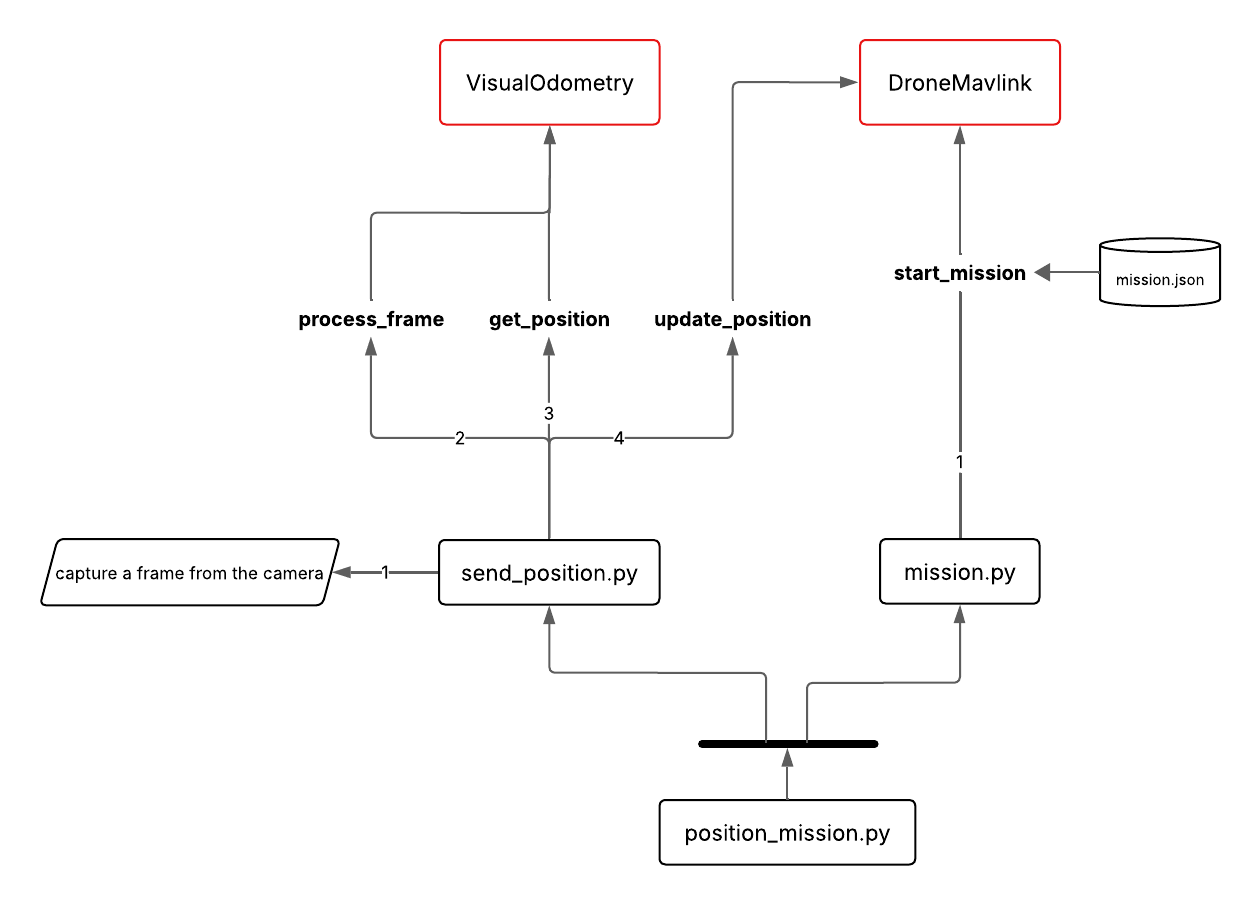
\includegraphics[width=1\textwidth, trim={0 0 0 0}, clip]{immagini/schema_software.png}
	\caption{Schema dell'architettura software e visualizzazione del flusso delle informazioni tra i moduli del sistema.}
	\label{fig:schema_software}
\end{figure}

\section{Mission}
La gestione della missione è stata imlementata utilizzando la modalità Offboard di PX4\footnote{\url{https://docs.px4.io/main/en/flight_modes/offboard}}, controllata attraverso il protocollo MAVLink. A differenza delle missioni gestite direttamente dal controllore di volo attraverso QGroundControl, questa soluzione permette di avere maggiore libertà e controllo sul volo.\\
La missione è composta da una lista ordinata di target, ciascuno con le proprie caratteristiche. Il software si occupa di gesitre le diverse fasi della missione, dall'avvio fino al completamento, verificando il raggiungimento dei target e gestendo il passaggio da un punto all'altro.\\ \\

\subsection{Architettura}
La missione viene eseguita interamente dalla classe \texttt{DroneMavlink}. All'interno essa utilizza il modulo \texttt{mavsdk}\footnote{\url{http://mavsdk-python-docs.s3-website.eu-central-1.amazonaws.com/}}, un insieme di librerie che permettono di comunicare con i sistemi che utilizzano il protocollo MAVLink. \\
La classe \texttt{DroneMavlink} contiene una funzione chiamata \texttt{start\_mission} che richiede solamente un parametro, la missione da eseguire. Essa viene rappresentata da un dizionario contenente la lista di target (esempio nella Lst. \ref{lst:esempio_missione}).
\begin{lstlisting}[language=json, caption={Esempio di configurazione della missione}, label={lst:esempio_missione}]
	{
		"targets": [
			{
				"north_m": 0.0,
				"east_m": 0.0,
				"down_m": -1.5
			},
			{
				"north_m": 3.0,
				"east_m": 3.0,
				"down_m": -1.5,
				"hover_time_ms": 1000
			}
		]
	}
\end{lstlisting}
Il compito di \texttt{start\_mission} è quello di gestire tutte le fasi principali della missione. In ordine, si occupa di inizializzare il collegamento con il flight controller; fa dei controlli pre-volo e attende finchè il sistema non ha tutti i requisiti per decollare; avvia la modalità Offboard di PX4; fa decollare il drone, impostando come target il parametro \texttt{TAKEOFF\_TARGET} della classe \texttt{DroneMavlink}, ovvero un obiettivo predefinito che indica la posizione che il drone deve raggiungere per il decollo; successivamente vengono iterati e impostati come obiettivo tutti i target, uno ad uno; infine viene cambiata la modalità del drone da Offboard a Land, che permette di far atterrare il drone e di disarmarlo in automatico. \\
Non è stata utilizzata la modalità Takeoff di PX4 perché, con la soluzione implementata in questo sistema, è possibile sfruttate tutti i vantaggi di personalizzazione dei target. \\ \\
Nella sezione \ref{sec:archi:target} viene descritto come singolarmente il drone raggiunge ogni target; in particolare, viene spiegato come sono state implementate tutte le opzioni presentate nella Sez. \ref{sec:problema:missione}.

\subsection{Target}
\label{sec:archi:target}
La funzione che permette di raggiungere un target si chiama \texttt{move\_to}, e riceve come parametro una \texttt{NamedTuple} chiamata \texttt{Target}. La lista degli elementi, con i vari valori di default, è presente della Lst. \ref{lst:target}.
\begin{lstlisting}[style=pythonstyle, caption={Lista degli elementi che un Target ha}, label={lst:target}]
class Target(NamedTuple):
	north_m: float
	east_m: float
	down_m: float
	yaw_deg: float = 0.0
	hover_time_ms: int = 0
	expiration_time_s: float = None
	vel_m_s: float = None
\end{lstlisting}
Non è necessario approfondire singolarmente ogni campo della struttura. Quelli che meritano una maggiore attenzione sono come le modalità hoverpoint e waypoint del target vengono attivate e il loro funzionamento.
\subsubsection{Hoverpoint}
Questa modalità permette al drone di raggiungere il target e di attendere il suo stazionamento. La posizione desiderata viene definita dalle tre coordinate \texttt{north\_m}, \texttt{east\_m} e \texttt{down\_m}, espresse nel sistema di riferimento NED (Sez. \ref{sez:archi:vo:pos}).\\ \\
Nella Fig. \ref{fig:diag_flusso_hoverpoint} è presente lo schema che descrive il funzionamento base di questa modalità. La prima istruzione che viene inviata al drone è quella di raggiungere un certo obiettivo; questo viene fatto attraverso la funzione \texttt{set\_position\_ned}. Successivamente, vengono monitorate in sequenza posizione, velocità e yaw per vedere quando il drone converge verso il suo obiettivo, seguendo le tolleranze impostate nella classe \texttt{DroneMavlink}.
\begin{figure}[!htbp]
	\centering
	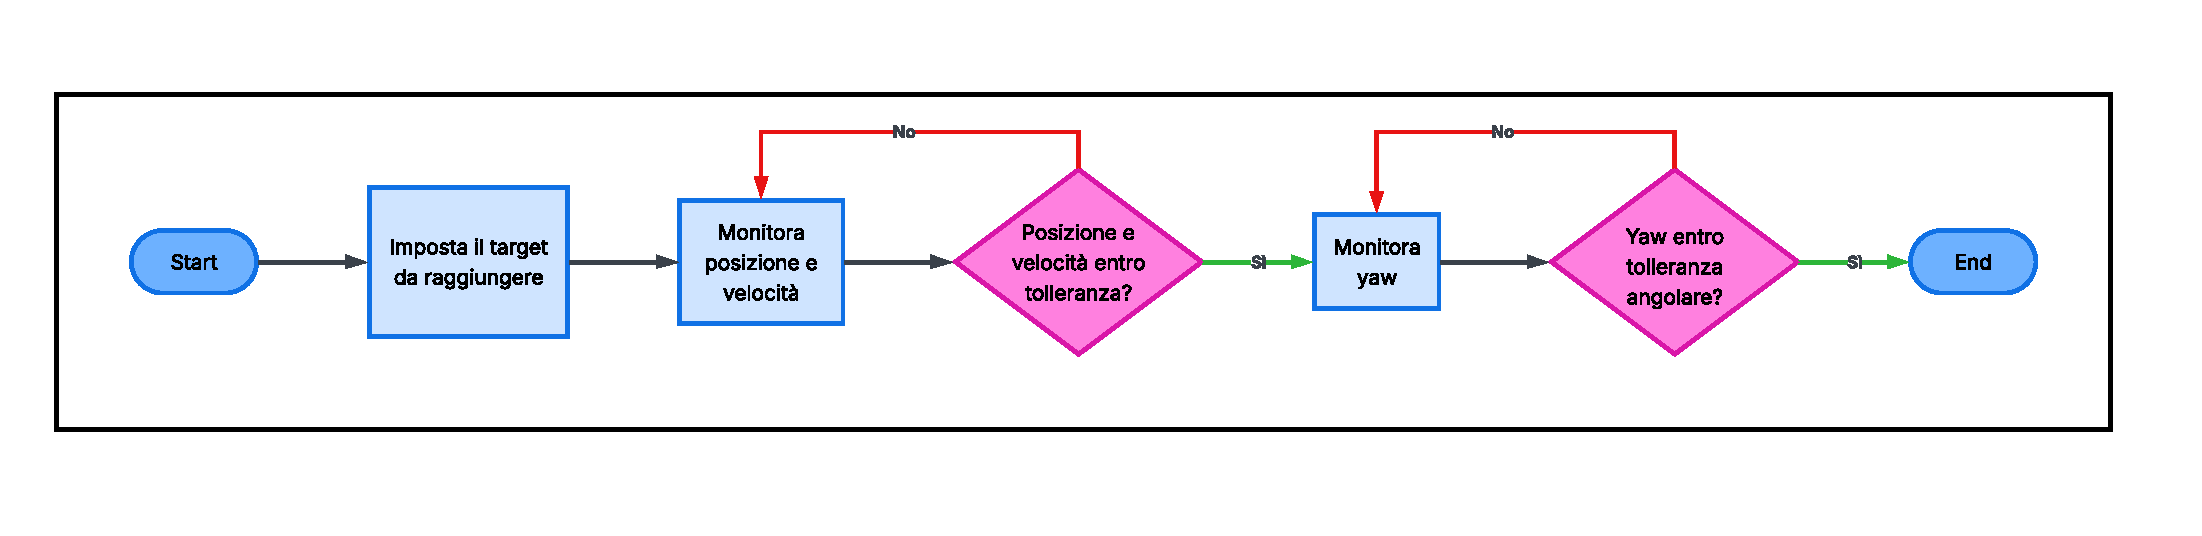
\includegraphics[width=0.95\textwidth, trim={0 0 0 0}, clip]{immagini/diagramma_flusso_hoverpoint.pdf}
	\caption{Diagramma di flusso della modalità hoverpoint di un target.}
	\label{fig:diag_flusso_hoverpoint}
\end{figure}

\subsubsection{Waypoint}
La modalità waypoint consente di raggiungere un obiettivo senza doversi fermare. È possibile creare un target che esegui questa modalità impostando uno dei due parametri \texttt{expiration\_time\_s} o \texttt{vel\_m\_s}. Essi indicano direttamente la velocità NED di dove il drone deve andare (usando alla funzione \texttt{set\_velocity\_ned}) e per quanto tempo mantenerla.  \\ \\
Nella Fig. \ref{fig:diag_flusso_waypoint} è rappresentato un diagramma di flusso del funzionamento base della modalità waypoint. Le parti che meritano un approfondimento sono due: il secondo blocco di decisione, dove vengono separati i vari calcoli delle velocità nei casi in cui si utilizza \texttt{expiration\_time\_s} da quello di \texttt{vel\_m\_s}; e l'ultimo blocco istruzione, dove viene dato il comando di impostare le coordinate NED della posizione.

\begin{figure}[!htbp]
	\centering
	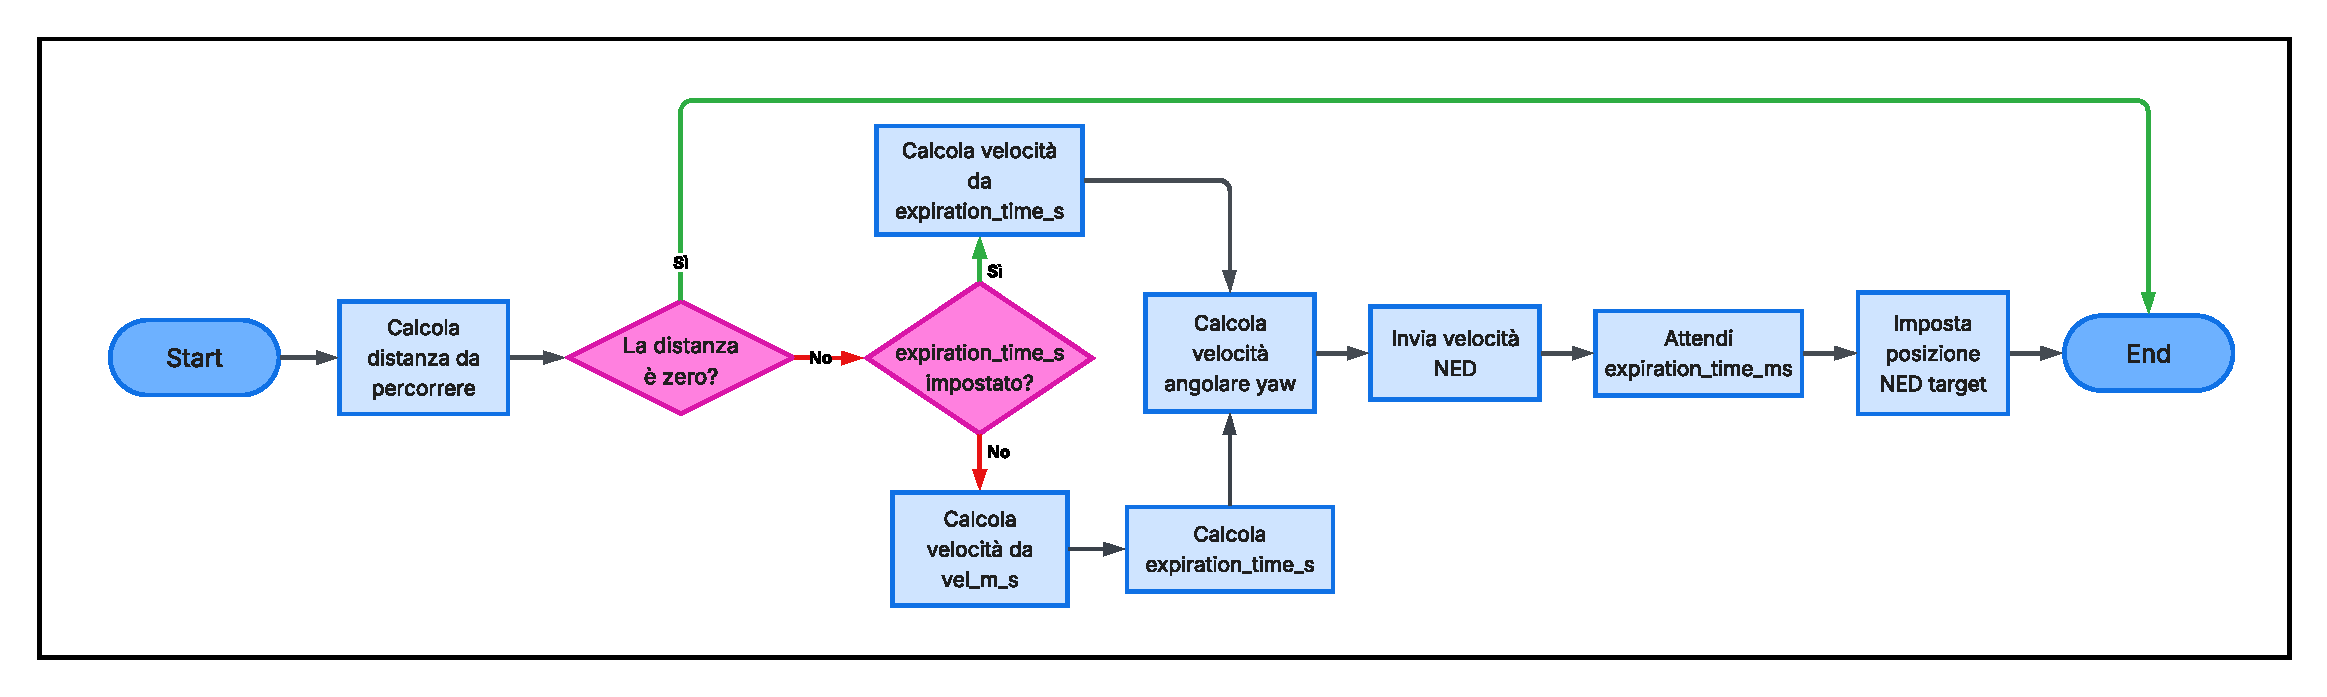
\includegraphics[width=1\textwidth, trim={0 0 0 0}, clip]{immagini/diagramma_flusso_waypoint.pdf}
	\caption{Diagramma di flusso della modalità waypoint di un target.}
	\label{fig:diag_flusso_waypoint}
\end{figure}

\paragraph{expiration\_time\_s} Avendo impostato il tempo che il drone ci mette per raggiungere il suo obiettivo ($t_\mathrm{exp\_time}$), la velocità per ogni coordinata si può calcolare in modo molto semplice facendo:
\[
\begin{bmatrix}
	v_N \\
	v_E \\
	v_D
\end{bmatrix}
=
\frac{1}{t_\mathrm{exp\_time}}
\cdot
\begin{bmatrix}
	\Delta N \\
	\Delta E \\
	\Delta D
\end{bmatrix}
\]

\paragraph{vel\_m\_s} Per calcolare la velocità NED partendo dalla velocità di crociera desiderata ($v_\mathrm{target}$), bisogna inanzitutto calcolare la distanza:
\[
d =
\sqrt{
	\Delta N^2 +
	\Delta E^2 +
	\Delta D^2
}
\]
Definiamo il vettore $\Delta p$, che indica la distanza tra il vecchio e il nuovo target:
\[
\Delta p =
\begin{bmatrix}
	\Delta N \\
	\Delta E \\
	\Delta D
\end{bmatrix}
\]
Non possiamo assegnare direttamente $v_\mathrm{target}$ in modo uguale per ogni coordinata. Quindi, dobbiamo distribuirla in modo proporzionale allo spostamento. Per fare ciò, dividiamo il vettore $\Delta p$ per la distanza calcolata precedentemente:
\[
\hat{u} =
\frac{\Delta p}{d}
\]
Successivamente, la velocità NED si può calcolare in questo modo:
\[
\begin{bmatrix}
	v_N \\
	v_E \\
	v_D
\end{bmatrix}
=
v_\mathrm{target}\cdot \hat{u}
\]
L'altro parametro necessario per il sistema è $t_\mathrm{exp\_time}$:
\[
t_\mathrm{exp\_time} = \frac{d}{v_\mathrm{target}}
\]

\paragraph{Comando posizione finale} Per concludere, il comando \texttt{set\_velocity\_ned} imposta la velocità nelle varie coordinate NED del drone, senza mai fermarsi. È per questo che viene inviato il comando \texttt{set\_position\_ned} alla fine del blocco di codice, per evitare problematiche di questo tipo. Un possibile problema reale lo si potrebbe riscontrare nel caso in cui l'ultimo target della missione è un target di questo tipo, quindi il drone inizia la manovra di atterraggio e potrebbe cadere, dato che atterra mentre è in movimento; oppure nel caso in cui viene impostato anche il parametro \texttt{hover\_time\_ms} (un utilizzo insolito, ma comunque possibile).

\section{Visual odometry}
L'architettura della VO si può dividere in due parti: software e hardware. In questa sezione vengono affrontati entrambi gli aspetti, approfondendo principalmente l'architettura nel drone reale.

\subsection{Cattura e analisi del frame}
È stato scelto il modulo Python \texttt{picamera2}\footnote{\url{https://pip-assets.raspberrypi.com/categories/652-raspberry-pi-camera-module-2/documents/RP-008156-DS-7-picamera2-manual.pdf}} per l'acquisizione dei frame dalla camera. Nella Sez. \ref{sec:vo:camera} viene approfondita la configurazione dei vari parametri della camera. In particolare, viene utilizzata la funzione \texttt{picamera2.capture\_request} in modalità asincrona, impostando il parametro \texttt{signal\_function}; in questo modo, quando il frame è disponibile, verrà automaticamente richiamata la funzione impostata nel parametro \texttt{signal\_function}, che si occuperà di elaborare il frame e inviare i dati al flight controller. \\
Un diagramma di flusso che rappresenta l'implementazione di questa funzione è presente nella Fig. \ref{fig:diag_flusso_frame_an}. 
\begin{figure}[!htbp]
	\centering
	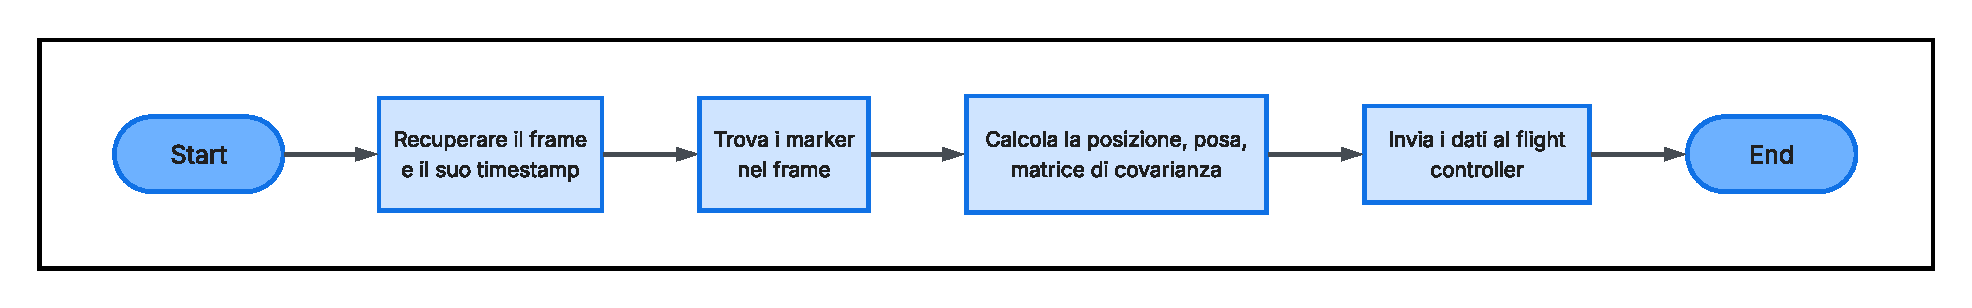
\includegraphics[width=1\textwidth, trim={0 0 0 0}, clip]{immagini/diagramma_flusso_frame_analyzer.pdf}
	\caption{Diagramma di flusso della funzione richiamata dal modulo \texttt{picamera2} per l'analisi del frame.}
	\label{fig:diag_flusso_frame_an}
\end{figure} \\
Prima di approfondire i calcoli di posizione, posa e della matrice di covarianza bisogna fare una considerazione sui marker, ovvero stabilire che azione intraprendere in caso l'immagine contenga più di un marker. Le principali opzioni disponibili sono tre: analizzare tutti i marker presenti, analizzarne alcuni, oppure analizzarne uno in particolare. \\
È stata scelta l'ultima opzione, perchè consente di effettuare la VO mantenendo una frequenza di calcolo abbastanza costante. I marker candidati vengono ordinati secondo la grandezza della propria superficie, in ordine decrescente. Il calcolo dell'area dei marker è stata eseguita utilizzando la formula dell'area di Gauss (chiamata anche Shoelace Formula o Green’s Formula)\footnote{\url{https://www.baeldung.com/cs/2d-polygon-area}}. \\
Infine, è stata aggiunta la possibilità di avere marker con dimensione diversa nello stesso ambiente. Questo consente di risolvere alcuni problemi di visibilità della camera o di aumentare la precisione del volo in alcune zone prestabilite.

\subsection{Calcolo della posizione}
\label{sez:archi:vo:pos}
Durante lo sviluppo del sistema di localizzazione, è stato necessario gestire la differenza tra i sistemi di riferimento; in particolare, il sistema della visione artificiale utilizza un sistema di coordinate ENU (East-North-Up), mentre il firmware PX4 utilizza il sistema NED (North-East-Down). Nella Fig. \ref{fig:enu_ned} è possibile visualizzarne la differenza. \\
\begin{figure}[!htbp]
	\centering
	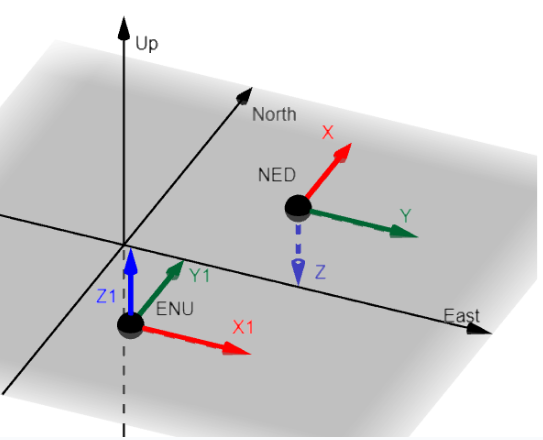
\includegraphics[width=0.5\textwidth, trim={0 0 0 0}, clip]{immagini/enu-ned.png}
	\caption{Rappresentazione dei sistemi di riferimento ENU e NED.}
	\label{fig:enu_ned}
\end{figure}
Per risolvere questo problema, è necessario convertire le coordinate da ENU a NED, applicando delle rotazioni. Osservando la Fig. \ref{fig:enu_ned}, è possibile notare che una delle combinazione di rotazioni che si possono applicare è: 90° sull'asse Z, 180° sull'asse Y. Quindi, sfruttando le matrici di rotazione Y e Z:
\[
R_y(\theta)=
\begin{bmatrix}
	\cos\theta & 0 & \sin\theta\\
	0 & 1 & 0\\
	-\sin\theta & 0 & \cos\theta
\end{bmatrix},
R_z(\psi)=
\begin{bmatrix}
	\cos\psi & -\sin\psi & 0\\
	\sin\psi & \cos\psi & 0\\
	0 & 0 & 1
\end{bmatrix}
\]
È possibile scrivere una matrice di conversione da ENU a NED:
\[
R_\mathrm{ENU\_NED}=R_y(\pi)\cdot R_z(\frac{\pi}{2})
\]
Essa deve essere applicata alla matrice di rotazione $R$, un valore ottenuto dalla funzione \texttt{solvePnP} di OpenCV che rappresenta come il marker è orientato rispetto alla camera. Questa funzione restituisce anche un vettore di traslazione $t$, che indica dove il marker di trova rispetto all'immagine. \\
\[
R_\mathrm{NED} = R\cdot R_\mathrm{ENU\_NED}
\]
Sia $p_m$ un vettore che rappresenta le coordinate a tre dimensioni di un punto nel mondo reale rispetto al marker; allora, le cordinate tridimensionali dello stesso punto nel sistema di riferimento della camera possiamo calcolarle in questo modo:
\[
p_c = R_\mathrm{NED}\cdot p_m+t
\]
Ma a noi interessa sapere l'opposto, ovvero trovare $p_m$:
\[
p_c = R_\mathrm{NED}\cdot p_m+t \Rightarrow p_c-t = R_\mathrm{NED}\cdot p_m \Rightarrow R_\mathrm{NED}^{-1}\cdot (p_c-t) = R_\mathrm{NED}^{-1}\cdot R_\mathrm{NED}\cdot p_m \Rightarrow
\]
\[
\Rightarrow p_m = R_\mathrm{NED}^{-1}\cdot (p_c-t)
\]
Una proprietà molto interessante della matrice di rotazione è che la sua inversa corrisponde alla sua trasposta: $R\cdot R^T=I$. Quindi è possibile semplificare la formula:
\[
p_m = R_\mathrm{NED}^T\cdot (p_c-t) = R_\mathrm{NED}^T\cdot p_c-R_\mathrm{NED}^T\cdot t
\]
In questo caso, il vettore $p_c$ punta all'origine della camera, quindi ha valore $\begin{bmatrix} 0 & 0 & 0 \end{bmatrix}^T$; di conseguenza, la formula diventa:
\[
p_m = R_\mathrm{NED}^T\cdot p_c-R_\mathrm{NED}^T\cdot t = R_\mathrm{NED}^T\cdot \begin{bmatrix} 0 & 0 & 0 \end{bmatrix}^T-R_\mathrm{NED}^T\cdot t = -R_\mathrm{NED}^T\cdot t
\]
Dentro questa formula manca ancora un'informazione, ovvero la posizione relativa del marker rispetto all'ambiente. Ognuno di essi si trova in una posizione diversa e nel calcolo della posizione questa informazione deve essere aggiunta. Per ogni marker, devono essere inserite le informazioni di posizione ENU, dimensione in metri e ID dentro un file json, che quindi descriverà l'ambiente della missione. \\
Definiamo $p_\mathrm{marker}$ il vettore posizione ENU del marker corrente, Allora, la formula precedente diventa:
\[
p_m = -R_\mathrm{NED}^T\cdot t + (R_\mathrm{ENU\_NED}\cdot p_\mathrm{marker})
\]
Riassumento:
\[
R_\mathrm{ENU\_NED}=R_y(\pi)\cdot R_z(\frac{\pi}{2})
\]
\[
R_\mathrm{NED} = R\cdot R_\mathrm{ENU\_NED}
\]
\[
\boxed{
		p_m = -R_\mathrm{NED}^T\cdot t + (R_\mathrm{ENU\_NED}\cdot p_\mathrm{marker})
}
\]
\subsection{Calcolo della posa}
Per descrivere l'orientamento del drone nello spazio tridimensionale è necessario analizzare la matrice $R_\mathrm{NED}$; in particolar modo, com'è composta \cite{kriz2006euler}. Partiamo dalla matrice di rotazione $R$. La possiamo descrivere attraverso le tre matrici di rotazione $X, Y, Z$:
\[
R_x(\phi)=
\begin{bmatrix}
	1 & 0 & 0\\
	0 & \cos\phi & -\sin\phi\\
	0  & \sin\phi & \cos\phi
\end{bmatrix},
R_y(\theta)=
\begin{bmatrix}
	\cos\theta & 0 & \sin\theta\\
	0 & 1 & 0\\
	-\sin\theta & 0 & \cos\theta
\end{bmatrix},
R_z(\psi)=
\begin{bmatrix}
	\cos\psi & -\sin\psi & 0\\
	\sin\psi & \cos\psi & 0\\
	0 & 0 & 1
\end{bmatrix}
\]
Adottando la convenzione ZYX, la matrice di rotazione $R$ si ottiene moltiplicando le matrici di rotazione nel seguente modo:
\[
R=R_z(\psi) \cdot R_y(\theta) \cdot R_x(\phi)
\]
Sviluppiamo prima il prodotto tra le matrici di rotazione $Y$ e $X$:
\[
R_yR_x=
\begin{bmatrix}
	\cos\theta & \sin\theta\sin\phi & \sin\theta\cos\phi\\
	0 & \cos\phi & -\sin\phi\\
	-\sin\theta & \cos\theta\sin\phi & \cos\theta\cos\phi
\end{bmatrix}
\]
Per poi unire anche la matrice relativa allo yaw:
\[
R=
\begin{bmatrix}
	\cos\psi & -\sin\psi & 0\\
	\sin\psi & \cos\psi & 0\\
	0 & 0 & 1
\end{bmatrix}
\cdot
\begin{bmatrix}
	\cos\theta & \sin\theta\sin\phi & \sin\theta\cos\phi\\
	0 & \cos\phi & -\sin\phi\\
	-\sin\theta & \cos\theta\sin\phi & \cos\theta\cos\phi
\end{bmatrix}=
\]
\[
\begin{bmatrix}
	\cos\psi\cos\theta &
	\cos\psi\sin\theta\sin\phi-\sin\psi\cos\phi &
	\cos\psi\sin\theta\cos\phi+\sin\psi\sin\phi\\
	\sin\psi\cos\theta &
	\sin\psi\sin\theta\sin\phi+\cos\psi\cos\phi &
	\sin\psi\sin\theta\cos\phi-\cos\psi\sin\phi\\
	-\sin\theta &
	\cos\theta\sin\phi &
	\cos\theta\cos\phi
\end{bmatrix}
\]
Abbiamo trovato $R$, quindi per calcolare $R_\mathrm{NED}$ basta moltiplicarla per la matrice di conversione $R_\mathrm{ENU\_NED}$:
\[
	R_\mathrm{NED} =
	R_\mathrm{ENU\_NED}
	\cdot
	\begin{bmatrix}
		\cos\psi\cos\theta &
		\cos\psi\sin\theta\sin\phi-\sin\psi\cos\phi &
		\cos\psi\sin\theta\cos\phi+\sin\psi\sin\phi\\
		\sin\psi\cos\theta &
		\sin\psi\sin\theta\sin\phi+\cos\psi\cos\phi &
		\sin\psi\sin\theta\cos\phi-\cos\psi\sin\phi\\
		-\sin\theta &
		\cos\theta\sin\phi &
		\cos\theta\cos\phi
	\end{bmatrix}
	=
\]
\[
\begin{bmatrix}
	0&1&0\\
	1&0&0\\
	0&0&-1
\end{bmatrix}
\cdot
\begin{bmatrix}
	\cos\psi\cos\theta &
	\cos\psi\sin\theta\sin\phi-\sin\psi\cos\phi &
	\cos\psi\sin\theta\cos\phi+\sin\psi\sin\phi\\
	\sin\psi\cos\theta &
	\sin\psi\sin\theta\sin\phi+\cos\psi\cos\phi &
	\sin\psi\sin\theta\cos\phi-\cos\psi\sin\phi\\
	-\sin\theta &
	\cos\theta\sin\phi &
	\cos\theta\cos\phi
\end{bmatrix}
=
\]
\[
\begin{bmatrix}
	\sin\psi\cos\theta &
	\sin\psi\sin\theta\sin\phi+\cos\psi\cos\phi &
	\sin\psi\sin\theta\cos\phi-\cos\psi\sin\phi\\
	\cos\psi\cos\theta &
	\cos\psi\sin\theta\sin\phi-\sin\psi\cos\phi &
	\cos\psi\sin\theta\cos\phi+\sin\psi\sin\phi\\
	\sin\theta &
	-\cos\theta\sin\phi &
	-\cos\theta\cos\phi
\end{bmatrix}
\]

\paragraph{Calcolo roll} L'angolo roll corrisponde alla misura di rotazione del sistema attorno all'asse X. In questo caso, l'asse da considerare non è l'asse X, ma l'asse Y, perché bisogna considerare che la matrice $R_\mathrm{NED}$ rappresenta la posizione e posa in coordinate NED, non ENU. Quindi, è possibile calcolarlo calcolando l'angolo $\theta$ in questo modo:
\[
\boxed{
	\theta = \arcsin({R_\mathrm{NED}}_{3,1}) = \arcsin(\sin\theta)
}
\]

\paragraph{Calcolo pitch} Sfruttando la stessa idea del calcolo del roll, si può calcolare il pitch. Essa corrisponde alla rotazione attorno all'asse Y, ma in questo caso, come spiegato precedentemente, corrisponde alla rotazione attorno all'asse X, ovvero l'angolo $\phi$. Di conseguenza:
\[
\boxed{
	\phi = \arctan(\frac{{R_\mathrm{NED}}_{3,2}}{{R_\mathrm{NED}}_{3,3}}) = \arctan(\frac{-\cos\theta\sin\phi}{-\cos\theta\cos\phi}) = \arctan(\frac{\sin\phi}{\cos\phi})
}
\]

\paragraph{Calcolo yaw} Infine, è possibile calcolare lo yaw calcolando $\psi$, ovvero la rotazione attorno all'asse Z. Guardando la matrice $R_\mathrm{NED}$, possiamo notare che:
\[
\psi=\arctan(\frac{{R_\mathrm{NED}}_{1,1}}{{R_\mathrm{NED}}_{2,1}})
\]
Dobbiamo fare attenzione ad un piccolo dettaglio, ovvero al senso di rotazione. Nel caso di roll e pitch cambiava l'asse, mentre in questo caso cambia il senso di rotazione, sempre per lo stesso motivo. Quindi, per risolvere questo conflitto dobbiamo inserire un segno $-$ nella formula per invertire il senso di rotazione e renderlo compatibile con lo yaw del flight controller:
\[
\boxed{
	\psi=\arctan(\frac{-{R_\mathrm{NED}}_{1,1}}{{R_\mathrm{NED}}_{2,1}})=\arctan(\frac{-\sin\psi\cos\theta}{\cos\psi\cos\theta})=\arctan(\frac{-\sin\psi}{\cos\psi})
}
\]

\subsection{Matrice di covarianza}
La matrice di covarianza permette di rappresentare l'incertezza delle variabili stimate dalla VO. Esse, insieme alla matrice di covarianza, vengono date in input al filtro di Kalman, che ne aggiornerà lo stato di conseguenza.

\subsubsection{Struttura}
Consideriamo il vettore di stato $\mathbf{s}$, una variabile aleatoria vettoriale composta in questo modo:
\[
\mathbf{s} =
\begin{bmatrix}
	x & y & z & \phi & \theta & \psi
\end{bmatrix}^{T}
\]
\begin{itemize}
	\item \(x,y,z\) rappresentano la posizione del drone nei tre assi cartesiani.
	\item\(\phi, \theta, \psi\) rappresentano rispettivamente roll, pitch e yaw.
\end{itemize}
Allora la matrice di covarianza $\mathbf{P}$ è formata in questo modo:
\[
\mathbf{P} =
\begin{bmatrix}
	\operatorname{Cov}(x,x) & \operatorname{Cov}(x,y) & \cdots & \operatorname{Cov}(x,\psi)\\
	\operatorname{Cov}(y,x) & \operatorname{Cov}(y,y) & \cdots & \operatorname{Cov}(y,\psi)\\
	\vdots & \vdots & \ddots & \vdots\\
	\operatorname{Cov}(\psi,x) & \operatorname{Cov}(\psi,y) & \cdots & \operatorname{Cov}(\psi,\psi)
\end{bmatrix}
\]
\\
Poiché la covarianza di una variabile con sé stessa coincide con la sua varianza:
\[
\operatorname{Cov}(x_i,x_i)
=\operatorname{Var}(x_i)
=\sigma_{x_i}^{2},
\]
la matrice può essere riscritta come:
\[
\mathbf{P} =
\begin{bmatrix}
	\sigma_x^2 & \operatorname{Cov}(x,y) & \cdots & \operatorname{Cov}(x,\psi) \\
	\operatorname{Cov}(y,x) & \sigma_y^2 & \cdots & \operatorname{Cov}(y,\psi) \\
	\vdots & \vdots & \ddots & \vdots \\
	\operatorname{Cov}(\psi,x) & \operatorname{Cov}(\psi,y) & \cdots & \sigma_\psi^2
\end{bmatrix}
\]
\\
Osservando il risultato, è possibile notare che questa è una matrice quadrata e simmetrica; questo vuol dire che per ogni coppia di indici (i,j), vale la relazione:
\[
P_{ij}=P_{ji}
\]
Questa proprietà deriva dalla simmetria della covarianza, per cui $\operatorname{Cov}(x_i,x_j)=\operatorname{Cov}(x_j,x_i)$.
\subsubsection{Calcoli}
In questa sezione vengono mostrati tutti i calcoli per ogni valore di posizione e posa.
Legenda (Fig. \ref{fig:dev_xy},\ref{fig:dev_z}):
\begin{itemize}
	\item $f$: distanza focale in pixel.
	\item $z_0$: asse ottico $z$ in metri.
	\item $O$: centro ottico.
	\item $pm$: piano immagine.
	\item $d'_x$: variazione nel piano immagine in pixel dell'asse X.
	\item $d_x$: variazione in metri di $d'_x$ nel mondo reale dell'asse X.
\end{itemize}
L'idea per calcolare la deviazione standard di ogni valore è trovare quanto esso cambia se l'immagine si sposta di 1 pixel.
\paragraph{Varianza x e y} Prendiamo in considerazione l'immagine in Fig. \ref{fig:dev_xy}; $d'_x$ rappresenta la variazione di $1px$ nel piano immagine $pm$, mentre $d_x$ rappresenta la distanza in metri rispetto alla variazione $d'_x$. \\
Osservango il disegno, è possibile notare che i triangoli $\triangle PM_0OPM_1$ e $\triangle L_0OL_1$ sono simili, dato che hanno due angoli congruenti; quindi, attraverso una proporzione è possibile dire che:
\[
\frac{d'_x}{f}=\frac{d_x}{z_0} \Rightarrow d_x=\frac{z_0}{f}\cdot d'_x
\]
Questa formula si chiama equazione prospettica. Sapendo che $d'_x=1px$, possiamo rappresentare la deviazione standard delle coordinate $x$ e $y$ in questo modo:
\[
\boxed{
	\sigma_x=\sigma_y=\frac{z_0}{f}\cdot 1px
}
\]
Infine, per ottenere la varianza basta elevare al quadrato la deviazione standard.

\begin{figure}[!htbp]
	\centering
	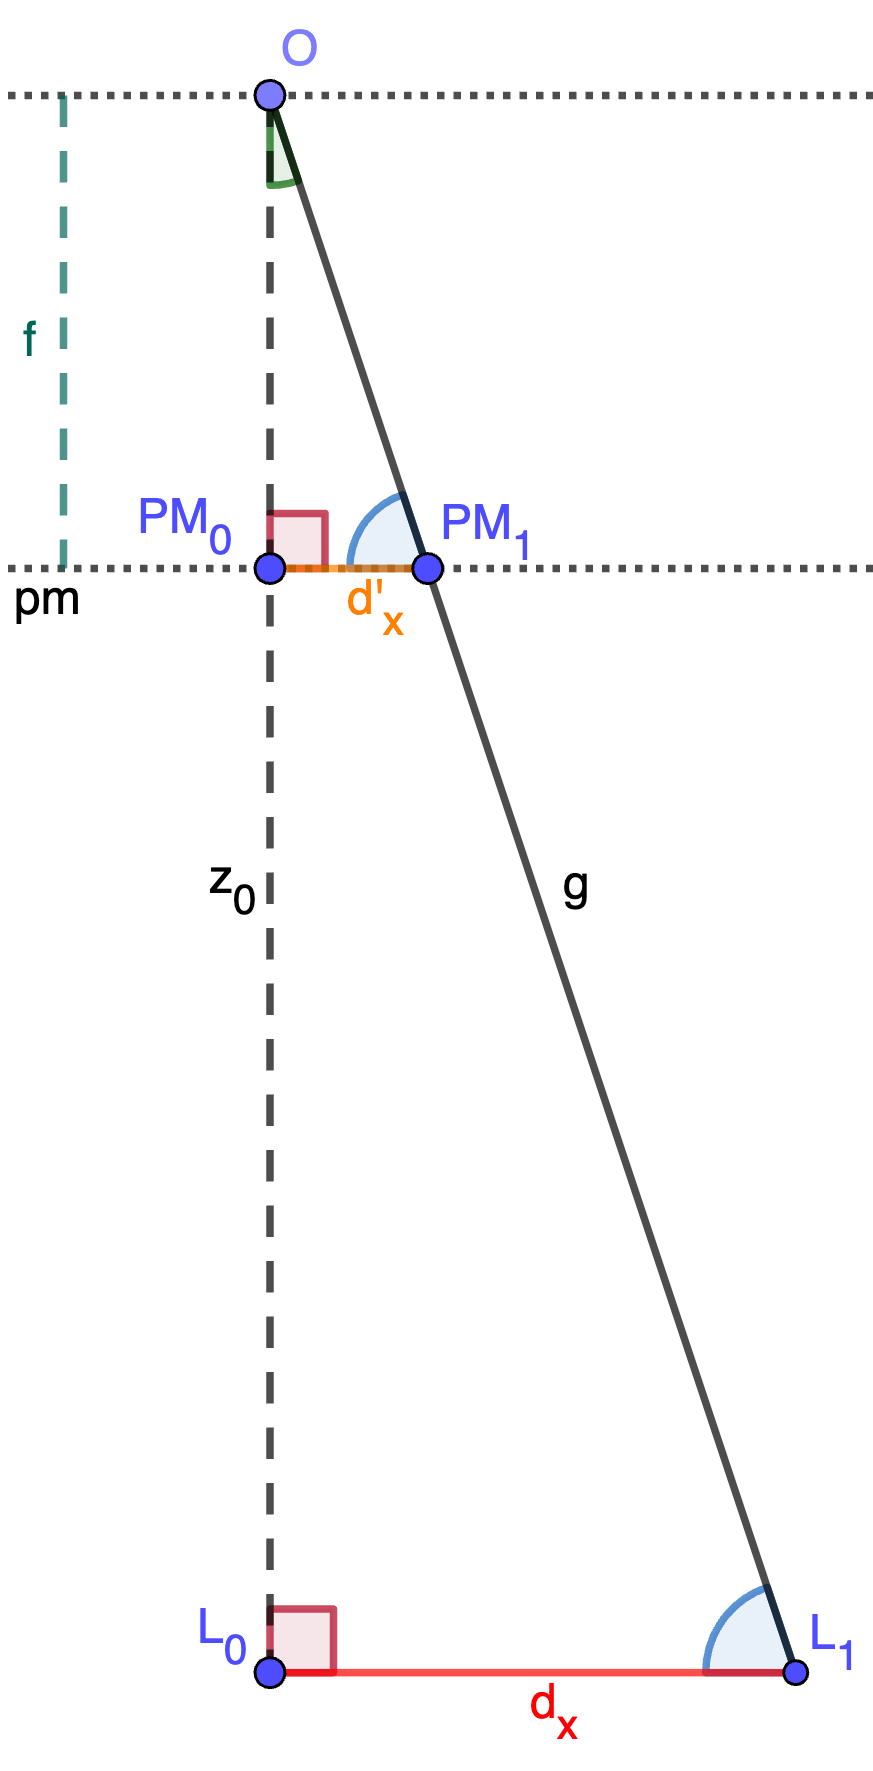
\includegraphics[width=0.3\textwidth, trim={0 0 0 0}, clip]{immagini/dev_xy.png}
	\caption{Disegno del calcolo della varianza delle coordinate $x$ e $y$.}
	\label{fig:dev_xy}
\end{figure}

\paragraph{Varianza z} La figura di riferimento è la Fig. \ref{fig:dev_z}. La deviazione standard è rappresentata dal segmento $d_z$. \\
Nella figura, possiamo notare che i triangoli $\triangle L_1AL_3$ e $\triangle L_0OL_3$ sono simili, dato che hanno due angoli congruenti. Attraverso lo stesso ragionamento, possiamo dire che anche i triangoli $\triangle FOPM_1$ e $\triangle L_0OL_3$ sono simili; quindi $\triangle FOPM_1$ e $\triangle L_1AL_3$ sono simili. Grazie a questo, possiamo scrivere la seguente proporzione:
\[
\frac{d_z}{d_x}=\frac{f}{\frac{l_{im}}{2}+d'_x} \Rightarrow d_z=\frac{f}{\frac{l_{im}}{2}+d'_x}\cdot d_x
\]
Il valore $d_x$ lo abbiamo calcolato nel paragrafo precedente, ed è uguale a $d_x=\frac{z_0}{f}\cdot d'_x$; mentre $d'_x=\frac{1}{2}px$, mezzo pixel per ogni lato del triangolo nel disegno. Quindi, sostituendo i valori, l'equazione risulta:
\[
d_z=\frac{f}{\frac{l_{im}}{2}+d'_x}\cdot d_x=\frac{f}{\frac{l_{im}}{2}+d'_x}\cdot\frac{z_0}{f}\cdot\frac{1}{2}px=\frac{z_0\cdot\frac{1}{2}px}{\frac{l_{im}}{2}+d'_x} = \frac{z_0\cdot\frac{1}{2}px}{\frac{l_{im}}{2}+\frac{1}{2}px} = \frac{z_0}{l_{im}+1px}
\]
Dato che il valore $l_{im}$ ha ordine di grandezza di qualche centinaio di pixel, è possibile eseguire la seguente approssimazione:
\[
\boxed{
	d_z=\frac{z_0}{l_{im}+1px} \approx \frac{z_0}{l_{im}}
}
\]
\begin{figure}[!htbp]
	\centering
	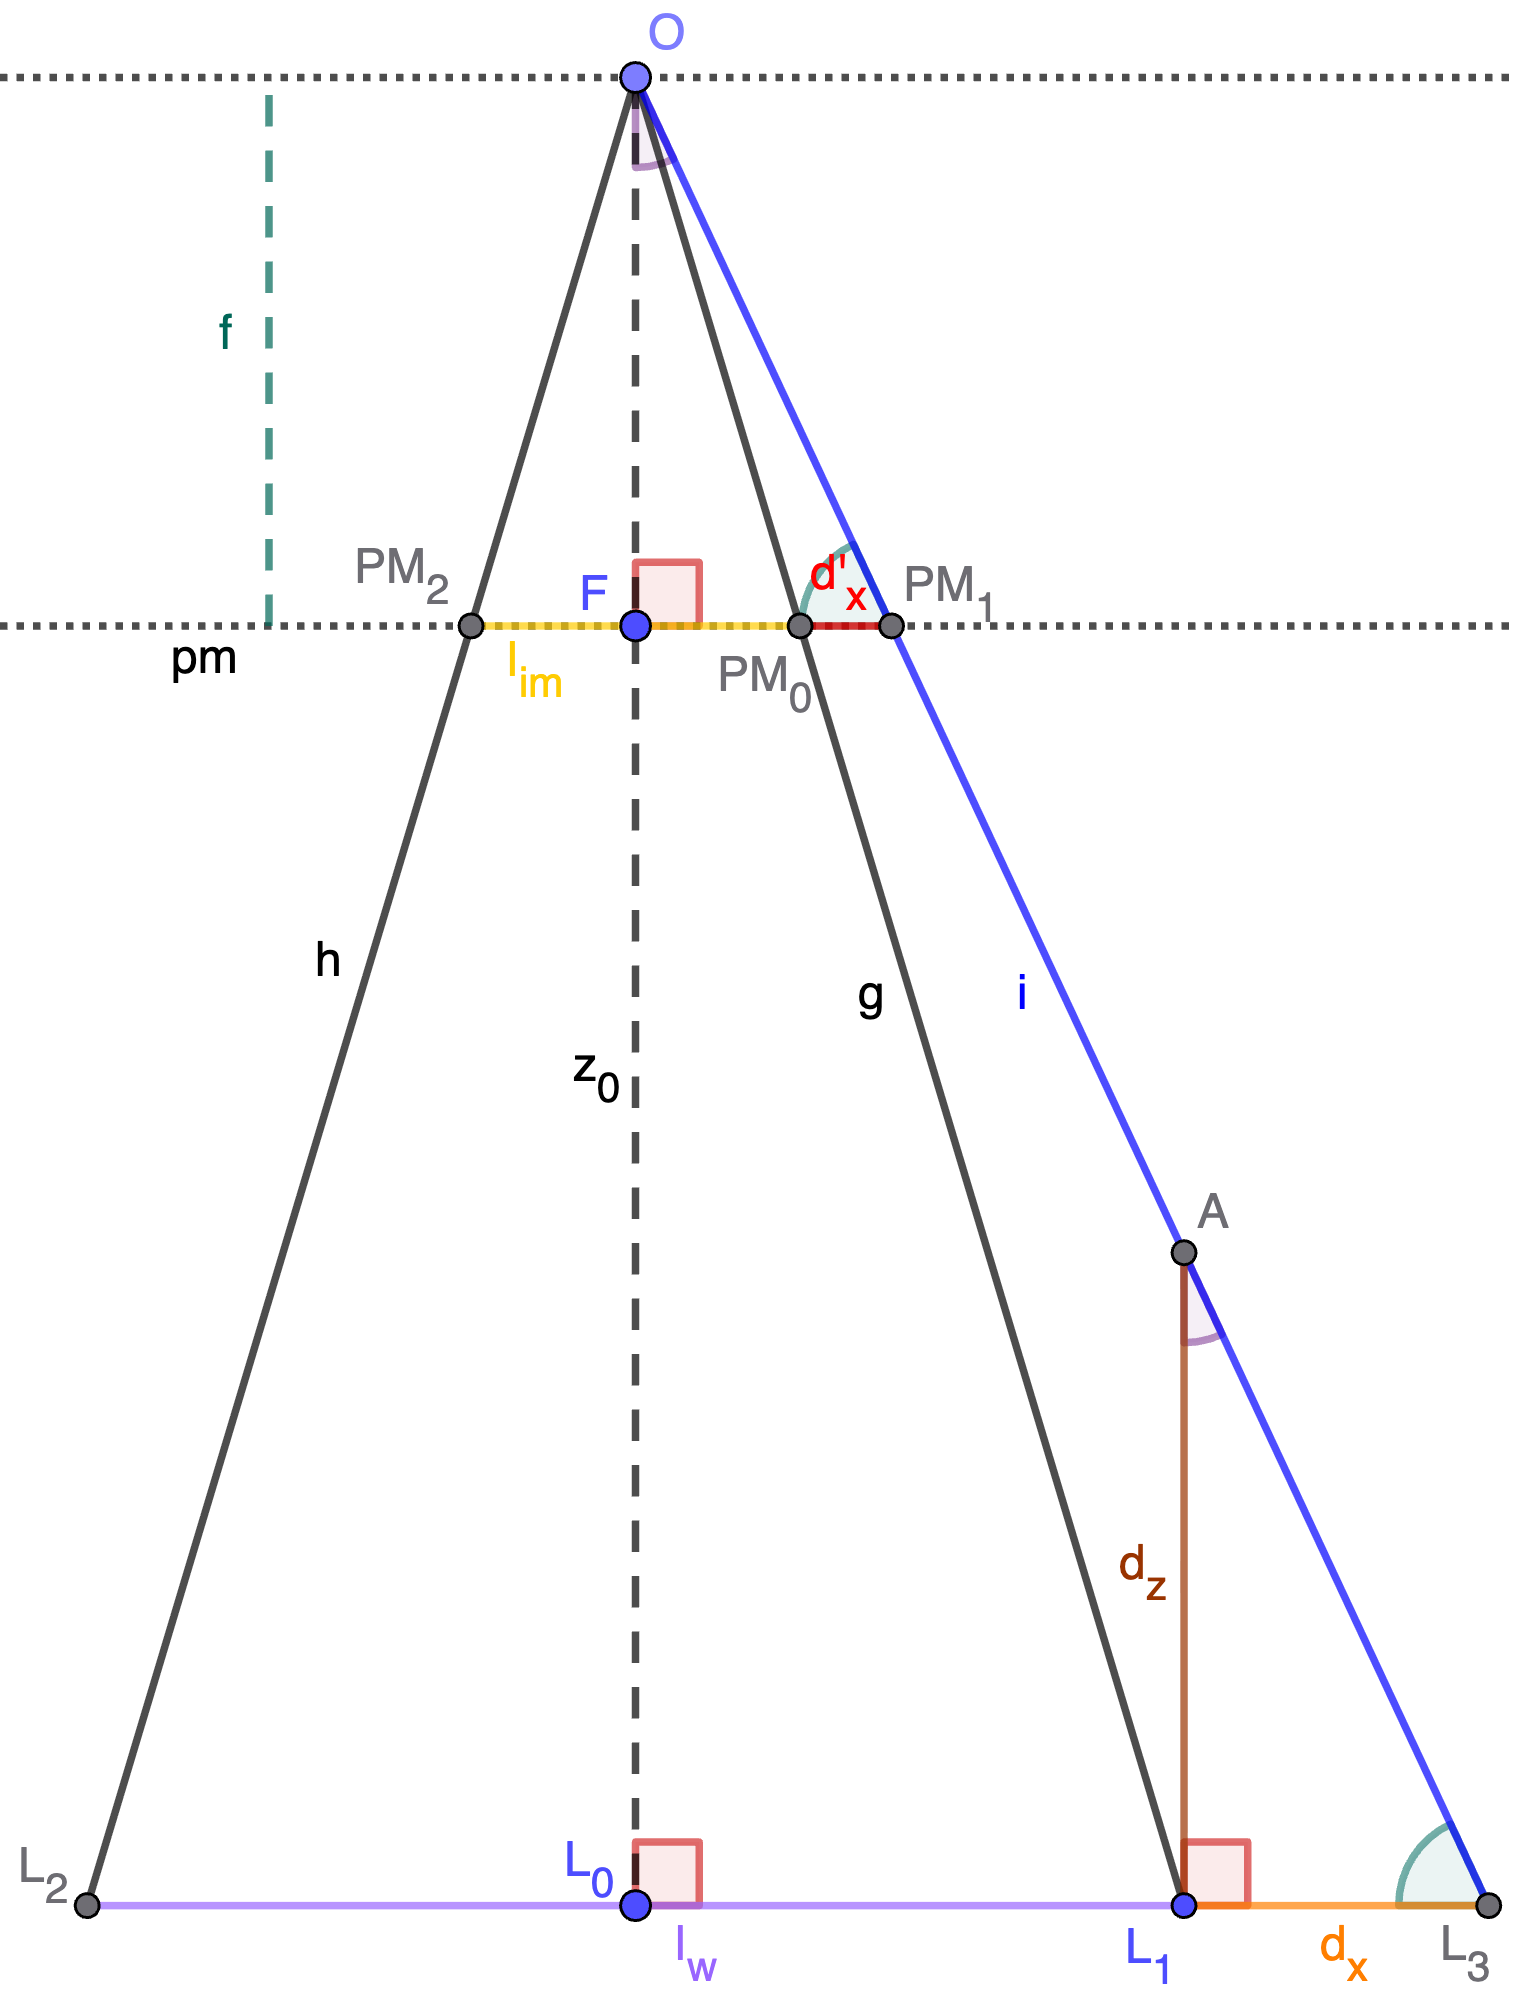
\includegraphics[width=0.4\textwidth, trim={0 0 0 0}, clip]{immagini/dev_z.png}
	\caption{Disegno del calcolo della varianza della coordinata $z$.}
	\label{fig:dev_z}
\end{figure}
\paragraph{Varianza roll e pitch} La deviazione standard è rappresentata dall'angolo $\gamma$, visibile in Fig. \ref{fig:dev_roll_pitch}. \\
Calcolare $d_x$ è molto semplice:
\[
d_x=m\cdot\tan(\gamma) \Rightarrow \tan(\gamma)=\frac{d_x}{m}
\]
Noi sappiamo che $d_x=1px$ e $m=\sqrt{f^2+(\frac{l_{im}}{2})^2}$, quindi:
\[
\tan(\gamma)=\frac{1}{\sqrt{f^2+(\frac{l_{im}}{2})^2}} \Rightarrow \gamma =\arctan(\frac{1}{\sqrt{f^2+(\frac{l_{im}}{2})^2}})
\]
Per valori di $x$ tendenti a 0, $\arctan(x) \approx x$, quindi:
\[
\boxed{
	\gamma=arctan(\frac{1}{\sqrt{f^2+(\frac{l_{im}}{2})^2}}) \approx \frac{1}{\sqrt{f^2+(\frac{l_{im}}{2})^2}}
}
\]

\begin{figure}[!htbp]
	\centering
	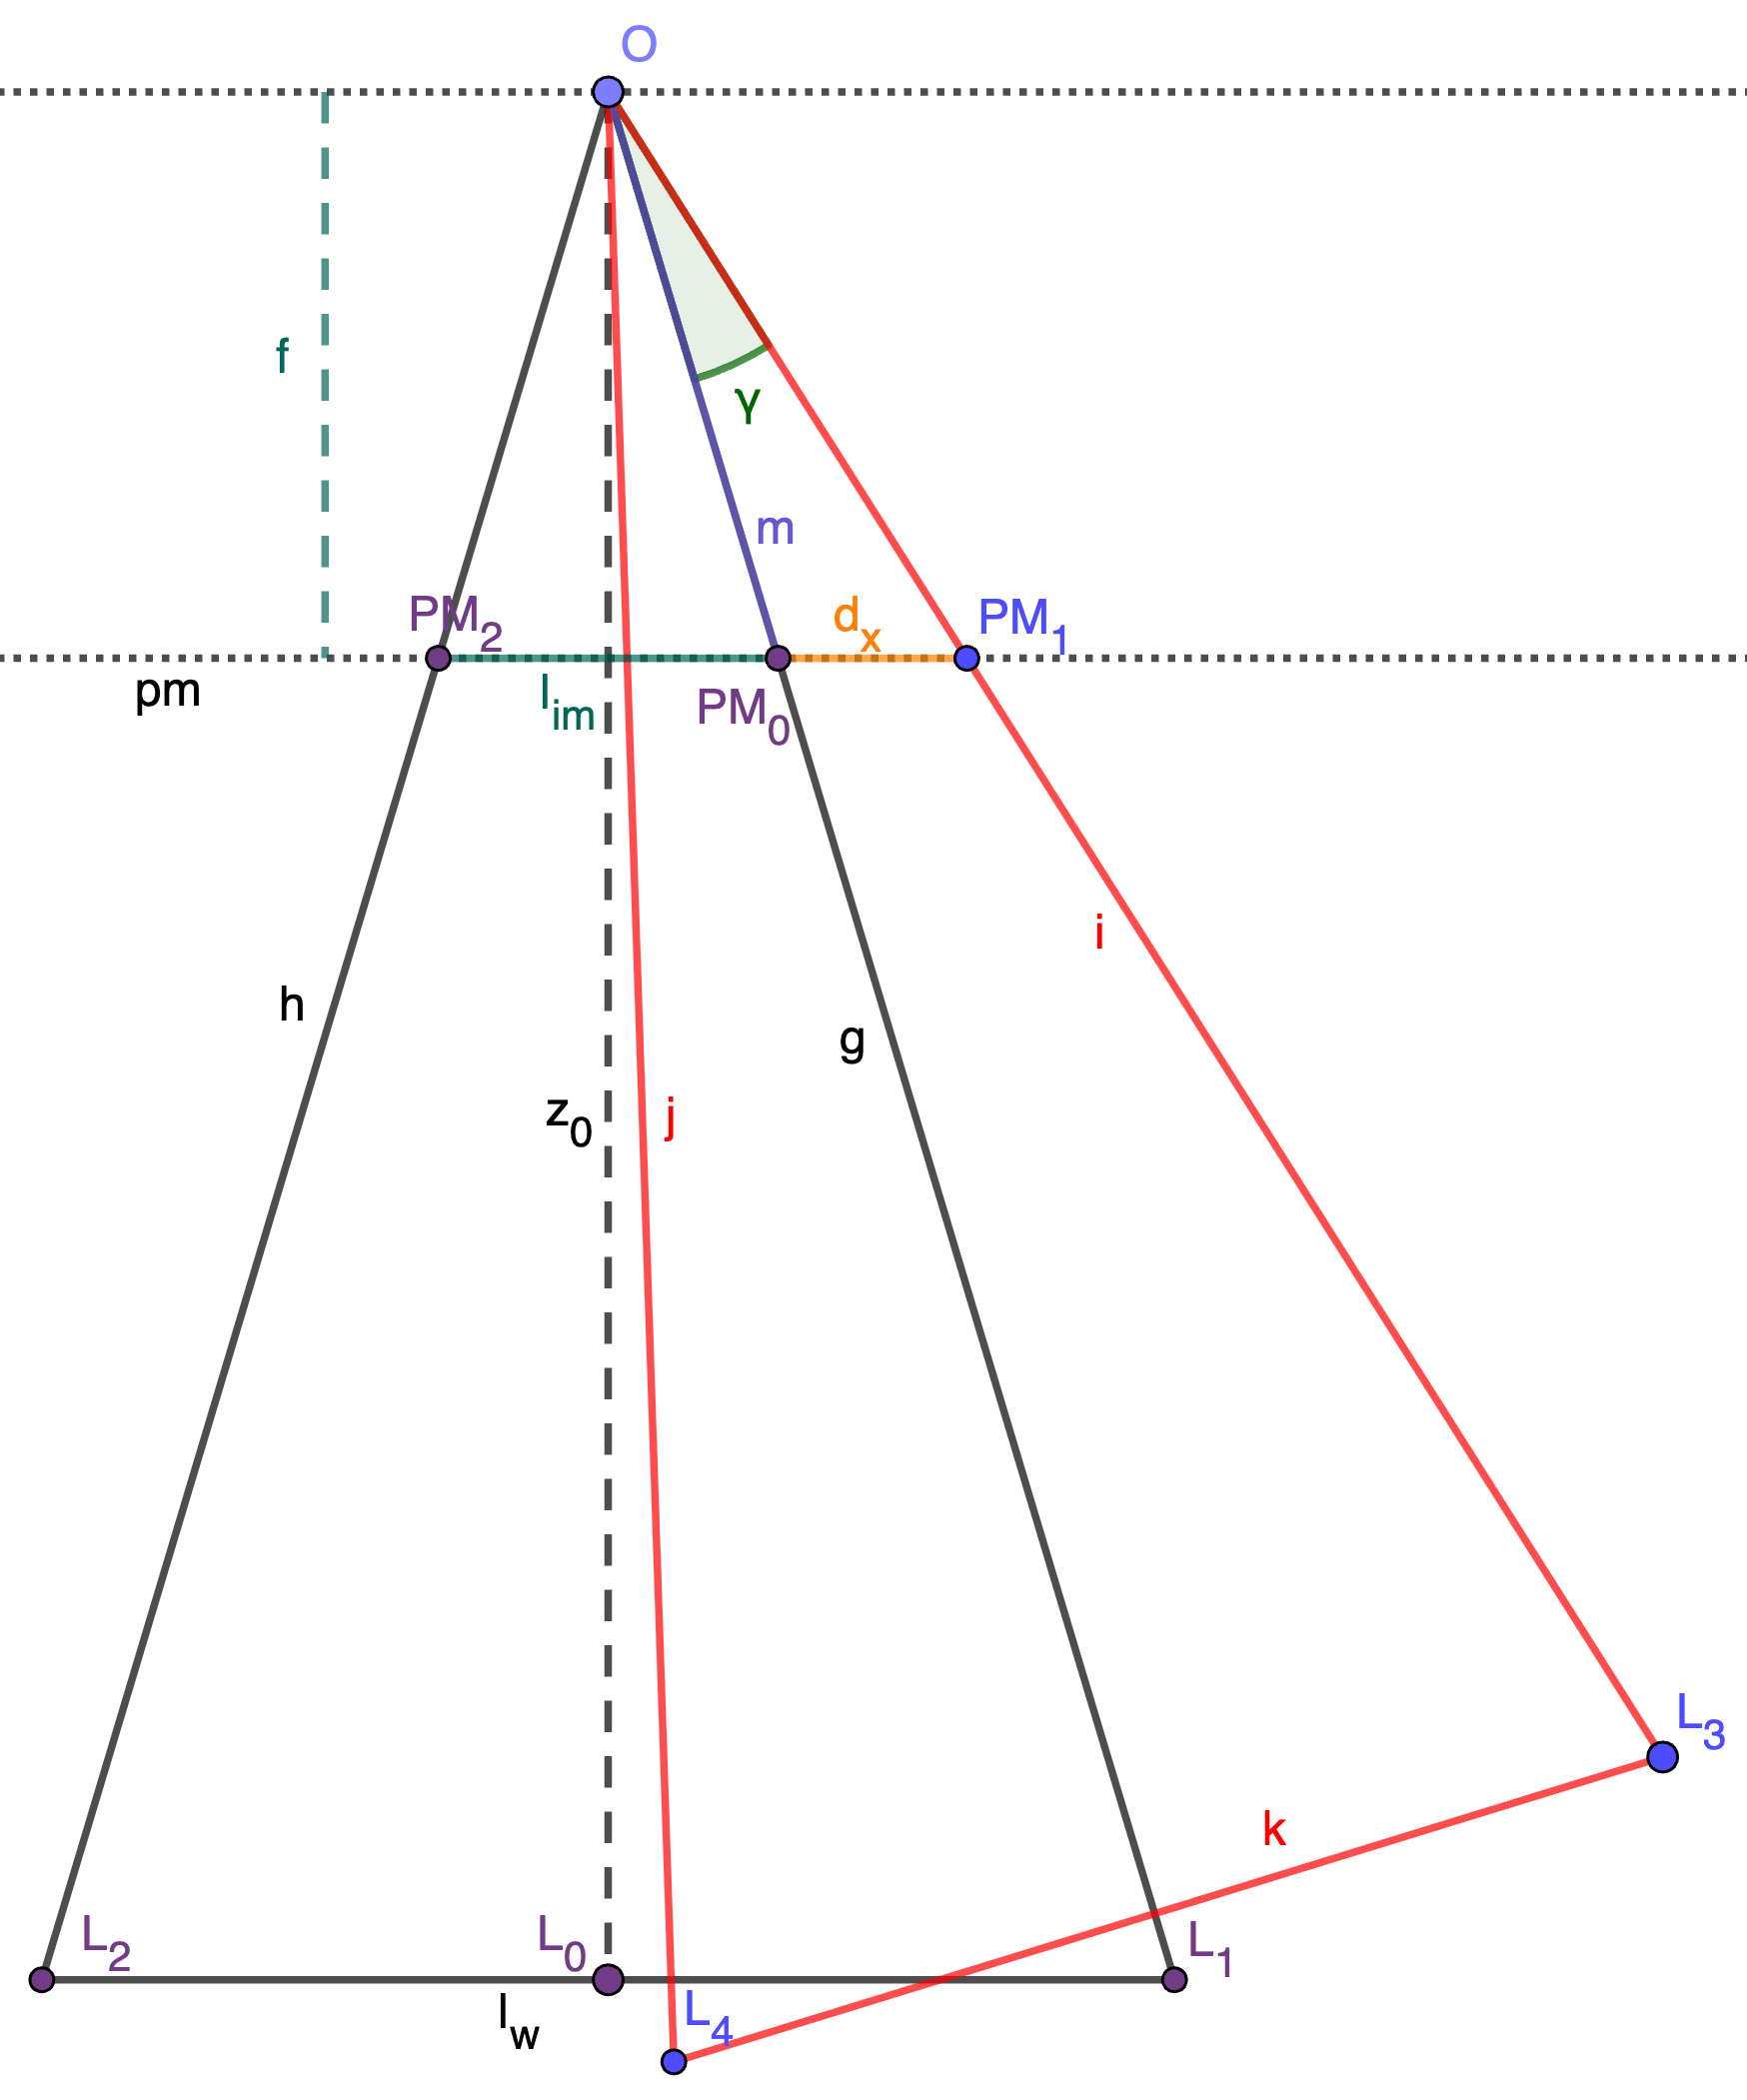
\includegraphics[width=0.5\textwidth, trim={0 0 0 0}, clip]{immagini/dev_roll_pitch.png}
	\caption{Disegno del calcolo della varianza degli angoli roll e pitch.}
	\label{fig:dev_roll_pitch}
\end{figure}

\paragraph{Varianza yaw} Nel disegno in Fig. \ref{fig:dev_yaw}, l'angolo $\alpha$ rappresenta la deviazione standard dello yaw. \\
Noi sappiamo che:
\[
 d_x=c\cdot\tan(\alpha)
\]
\[
c=\frac{\sqrt{l_0^2+l_0^2}}{2}=\frac{\sqrt{2}\cdot l_0}{2}=\frac{l_0}{\sqrt{2}}
\]
Quindi, sfruttando le formule precedenti, possiamo trovare $\alpha$ isolandolo dal $\tan(\alpha)$:
\[
tan(\alpha)=\frac{d_x}{c}=d_x\cdot\frac{\sqrt{2}}{l_0}
\]
Dalle premesse sappiamo che $d_x=1px$, quindi:
\[
\tan(\alpha)=\frac{\sqrt{2}}{l_0} \Rightarrow \alpha=\arctan(\frac{\sqrt{2}}{l_0})
\]
Dato che l'argomento di $\arctan(\frac{\sqrt{2}}{l_0})$ tente a 0, è possibile approssimare:
\[
\boxed{
	\alpha=\arctan(\frac{\sqrt{2}}{l_0})\approx \frac{\sqrt{2}}{l_0}
}
\]

\begin{figure}[!htbp]
	\centering
	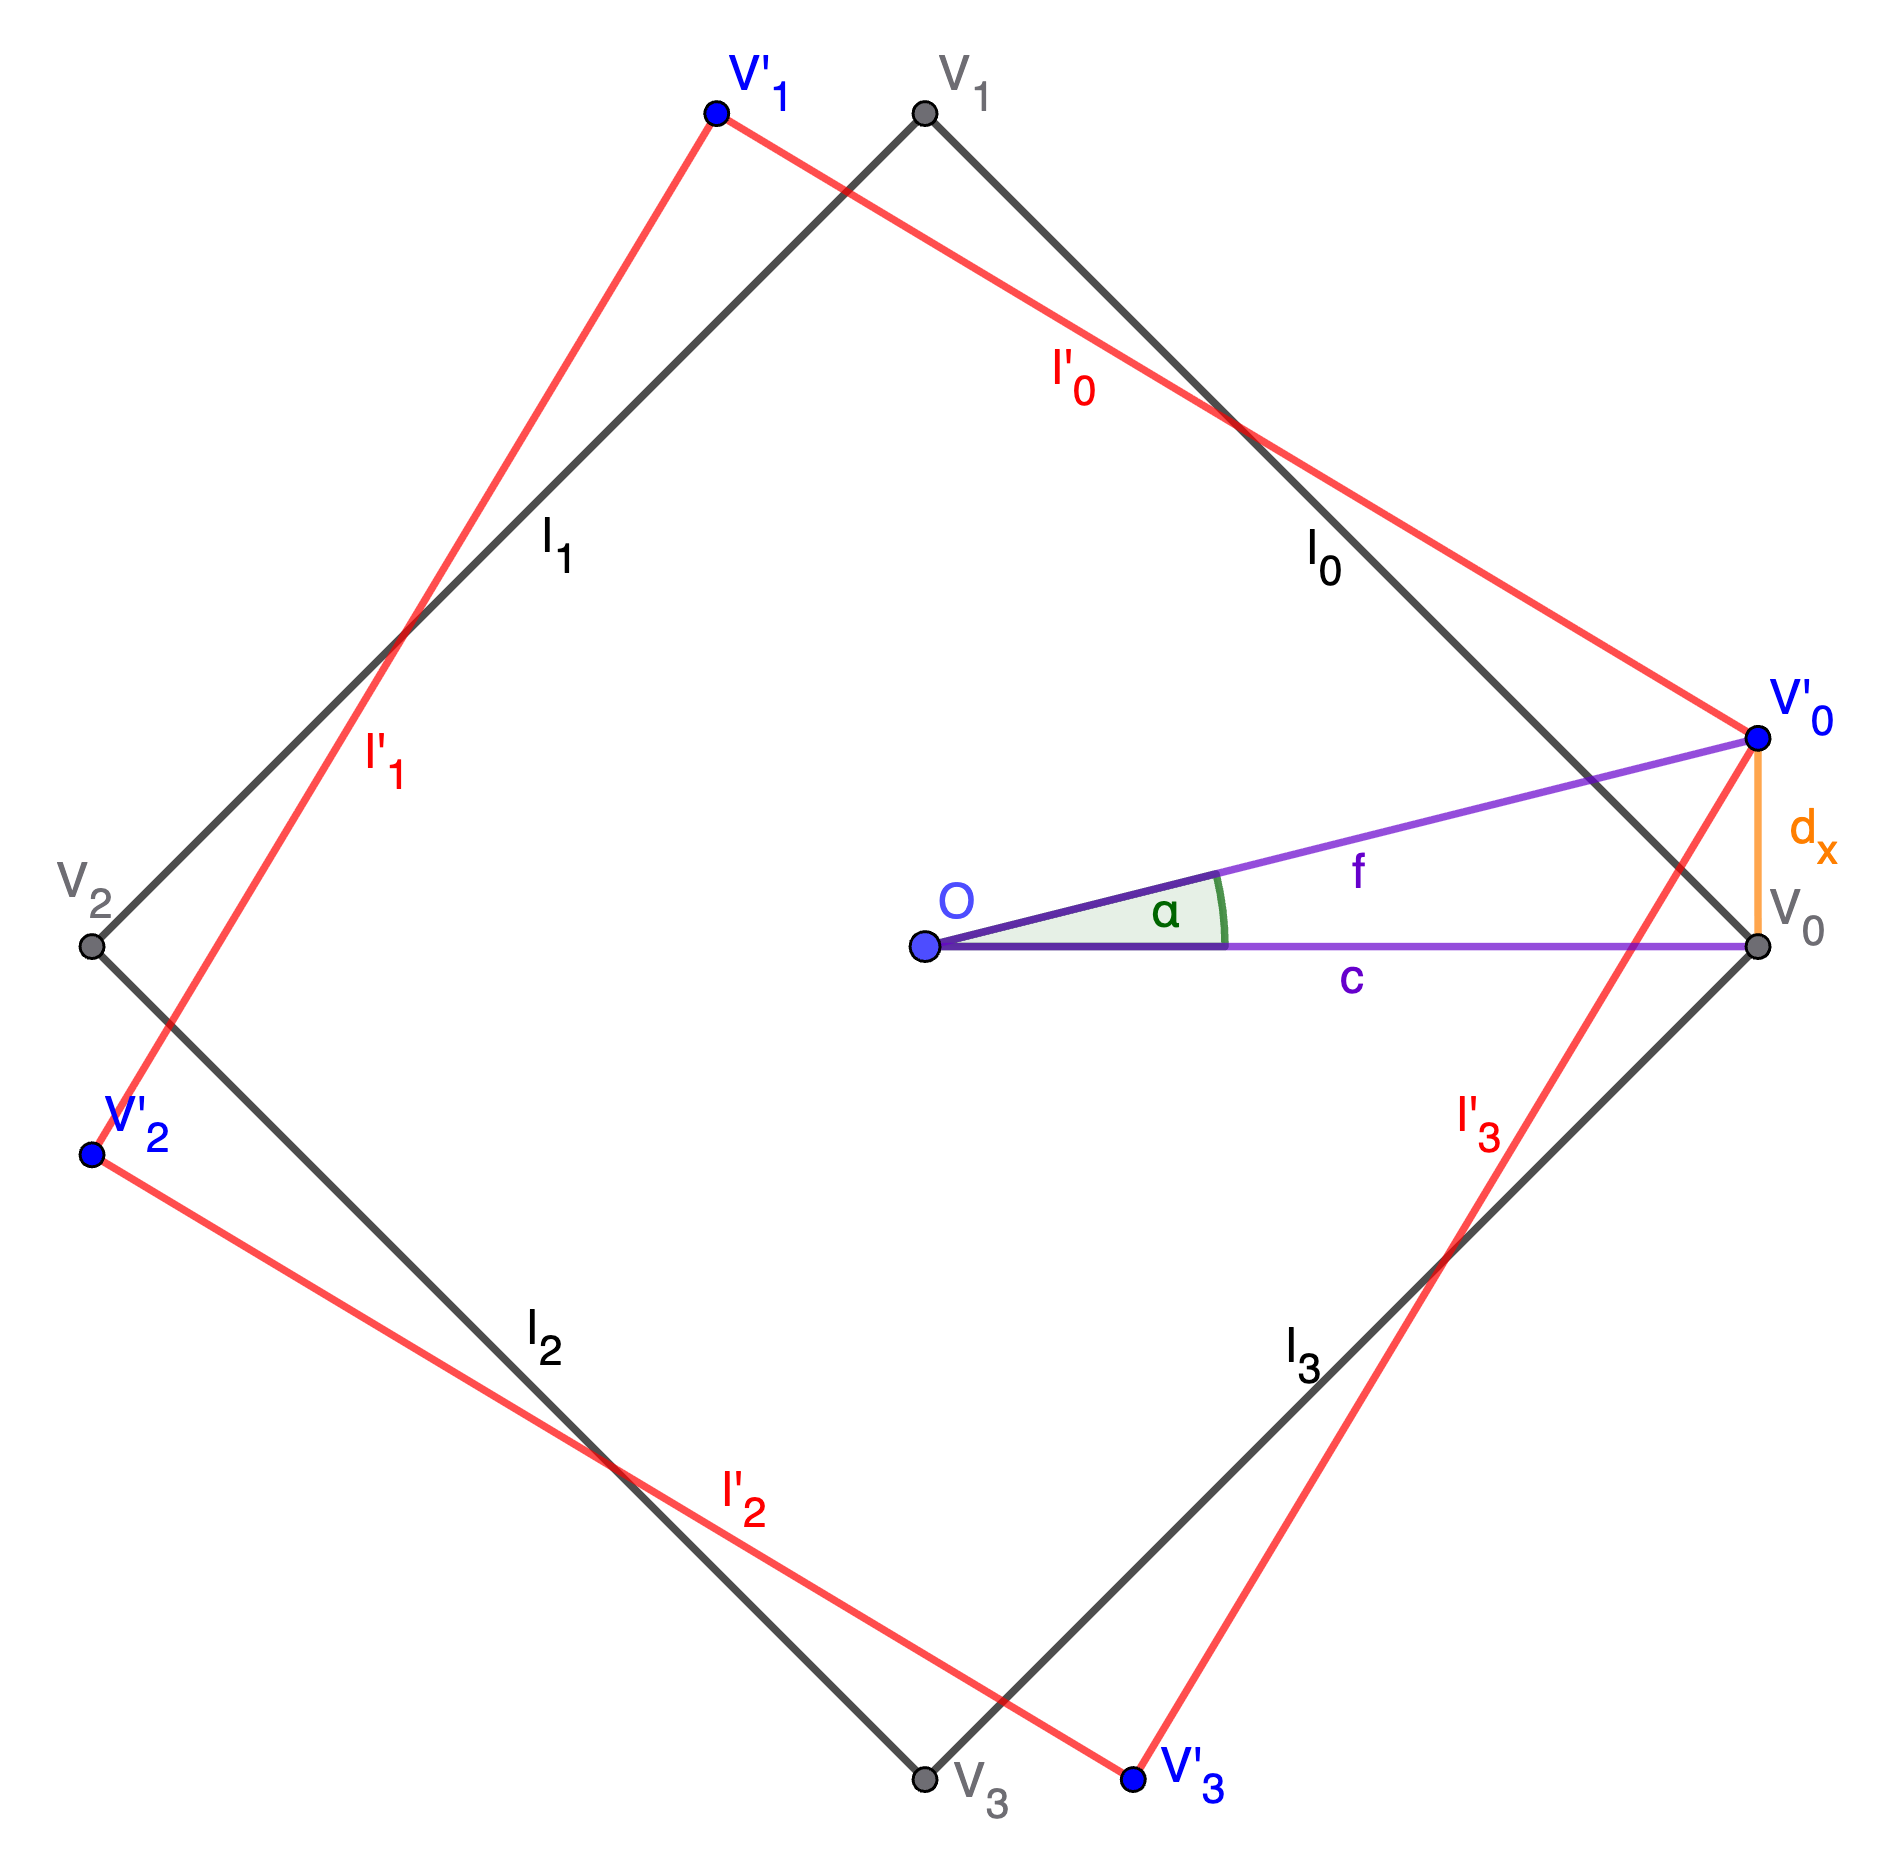
\includegraphics[width=0.5\textwidth, trim={0 0 0 0}, clip]{immagini/dev_yaw.png}
	\caption{Disegno del calcolo della varianza dell'angolo yaw.}
	\label{fig:dev_yaw}
\end{figure}
\subsubsection{Conclusioni}
Per concludere, nel modulo \texttt{mavsdk} la matrice di covarianza viene rappresentata attraverso la classe \texttt{mavsdk.mocap.Covariance}. Essa vuole come parametro \texttt{NaN}, se la matrice di covarianza è sconosciuta; opppure il triangolo superiore destro della matrice, dato che è simmetrica. Ecco confronto della matrice completa contro quella compressa:
\[
\mathbf{P} =
\begin{bmatrix}
	\sigma_x^2 & \operatorname{Cov}(x,y) & \cdots & \operatorname{Cov}(x,\psi) \\
	\operatorname{Cov}(y,x) & \sigma_y^2 & \cdots & \operatorname{Cov}(y,\psi) \\
	\vdots & \vdots & \ddots & \vdots \\
	\operatorname{Cov}(\psi,x) & \operatorname{Cov}(\psi,y) & \cdots & \sigma_\psi^2
\end{bmatrix}
\Rightarrow
\mathbf{P} =
\begin{bmatrix}
	\sigma_x^2 & \operatorname{Cov}(x,y) & \cdots & \operatorname{Cov}(x,\psi) \\
			 & \sigma_y^2 & \cdots & \operatorname{Cov}(y,\psi) \\
	 &  & \ddots & \vdots \\
	&  &  & \sigma_\psi^2
\end{bmatrix}
\]
La matrice originale ha $6x6$ valori, mentre quella compressa ne ha $21$. \\ \\
Infine, possiamo assumere che gli errori di misura dei sensori siano indipendenti tra loro. La covarianza tra due variabili indipentendi è zero, quindi la matrice finale sarà:
\[
\boxed{
	\mathbf{P} =
	\begin{bmatrix}
		\sigma_x^2 & 0 & \cdots & 0 \\
		& \sigma_y^2 & \cdots & 0 \\
		&  & \ddots & \vdots \\
		&  &  & \sigma_\psi^2
	\end{bmatrix}
}
\]

\subsection{Camera}
\label{sec:vo:camera}
\subsubsection{Scelta camera}
La scelta della camera ha un ruolo importantissimo per il sistema. I fattori importanti da considerare sono: la compatibilità con il Raspberry Pi 3, la risoluzione della camera, il FOV (Field of View) e il tipo di otturatore. I primi tre valori sono relativamente facili da soddisfare e dipendono fortemente dall'ambiente di volo; mentre l'ultimo è un fattore molto critico che richiede un pò di attenzione e approfondimento. \\
Esistono due tecnologie di otturatori: global shutter e rolling shutter. Nel primo caso, l'intera imagine viene acquisita nello stesso istante, pixel per pixel; mentre nel secondo caso, l'immagine viene acquisita riga per riga, quindi non nello stesso istante. Un esempio di rolling shutter camera è il Raspberry Pi Camera Module 2\footnote{\url{https://www.raspberrypi.com/products/camera-module-v2/}}. Il problema di quest'ultima tecnologia è che in caso di movimento laterale, l'immagine risulterà distorta (esempio in Fig. \ref{fig:rolling_shutter1}, \ref{fig:rolling_shutter2}. Notare come le linee dritte del pavimento si siano distorte). 
\begin{figure}[!htbp]
	\centering
	\begin{subfigure}[b]{0.48\textwidth}
		\centering
		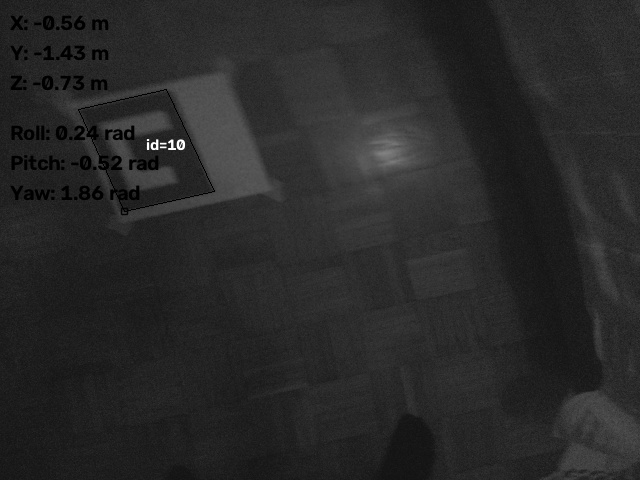
\includegraphics[width=\textwidth, trim={0 0 0 0}, clip]{immagini/rolling_shutter_1.jpg}
		\caption{Esempio distorsione verso destra.}
		\label{fig:rolling_shutter1}
	\end{subfigure}
	\hfill % Crea lo spazio orizzontale tra le due immagini
	\begin{subfigure}[b]{0.48\textwidth}
		\centering
		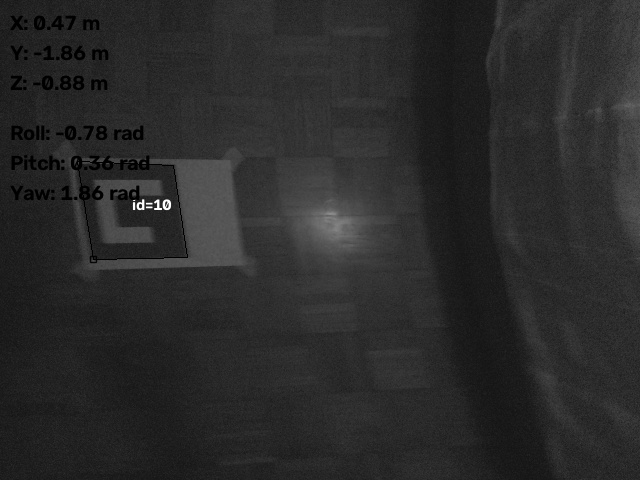
\includegraphics[width=\textwidth, trim={0 0 0 0}, clip]{immagini/rolling_shutter_2.jpg}
		\caption{Esempio distorsione verso sinistra.}
		\label{fig:rolling_shutter2}
	\end{subfigure}
	\caption{Distorsioni dovute dalla camera rolling shutter Raspberry Pi Camera Module 2. Le immagini sono state scattate nello stesso ambiente, con lo stesso pavimento.}
	\label{fig:rolling_shutter_all}
\end{figure}
Questa distorsione porta l'algoritmo della VO a restituire valori completamente sbagliati. Un esempio pratico dell'effetto di questo problema si può notare confrontanto i log nelle Fig. \ref{fig:log_rolling_shutter} e \ref{fig:log_global_shutter}; nella Fig. \ref{fig:log_rolling_shutter} è facile notare come ci siano degli sbalzi improvvisi, dovuti dalle immagini distorte della camera rolling shutter. Gli sbalzi si presentano soprattutto attraverso gli spostamenti laterali; infatti è proprio questo movimento che permette di accentuare questo fenomeno.
\begin{figure}[!htbp]
	\centering
	\begin{subfigure}[b]{0.48\textwidth}
		\centering
		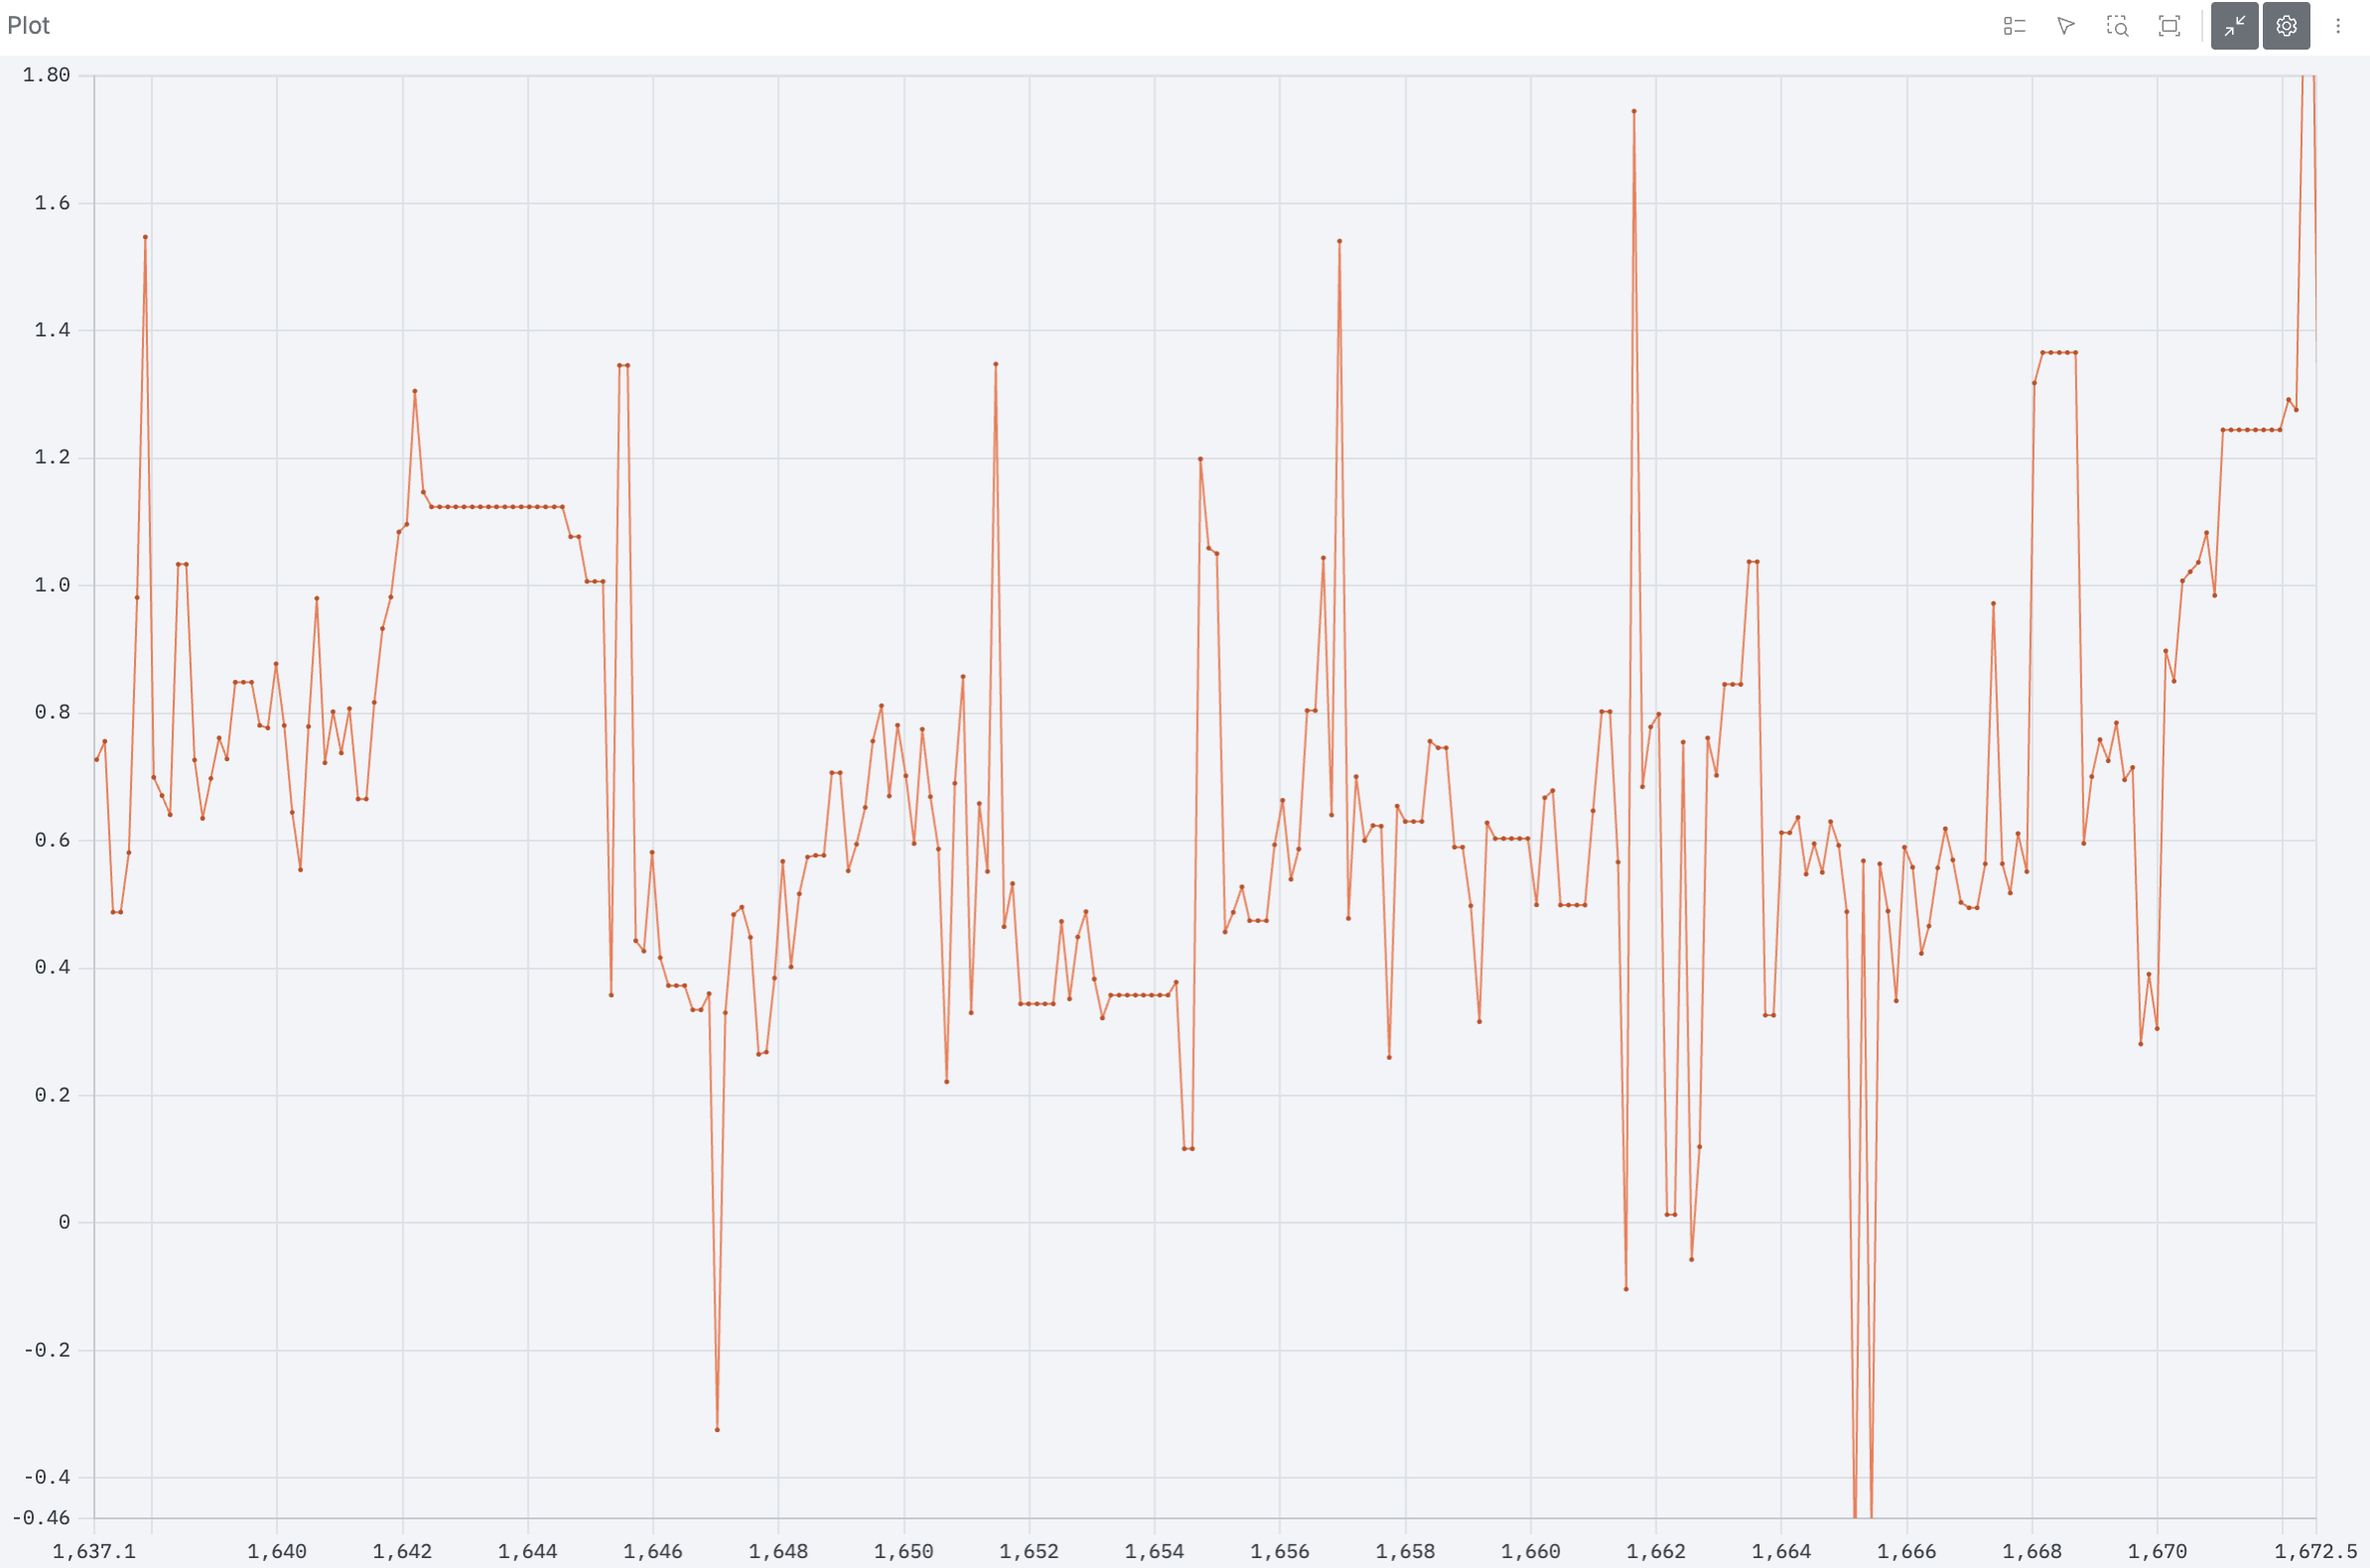
\includegraphics[width=\textwidth, trim={0 0 0 0}, clip]{immagini/log_distorto.png}
		\caption{Log con camera rolling shutter.}
		\label{fig:log_rolling_shutter}
	\end{subfigure}
	\hfill % Crea lo spazio orizzontale tra le due immagini
	\begin{subfigure}[b]{0.48\textwidth}
		\centering
		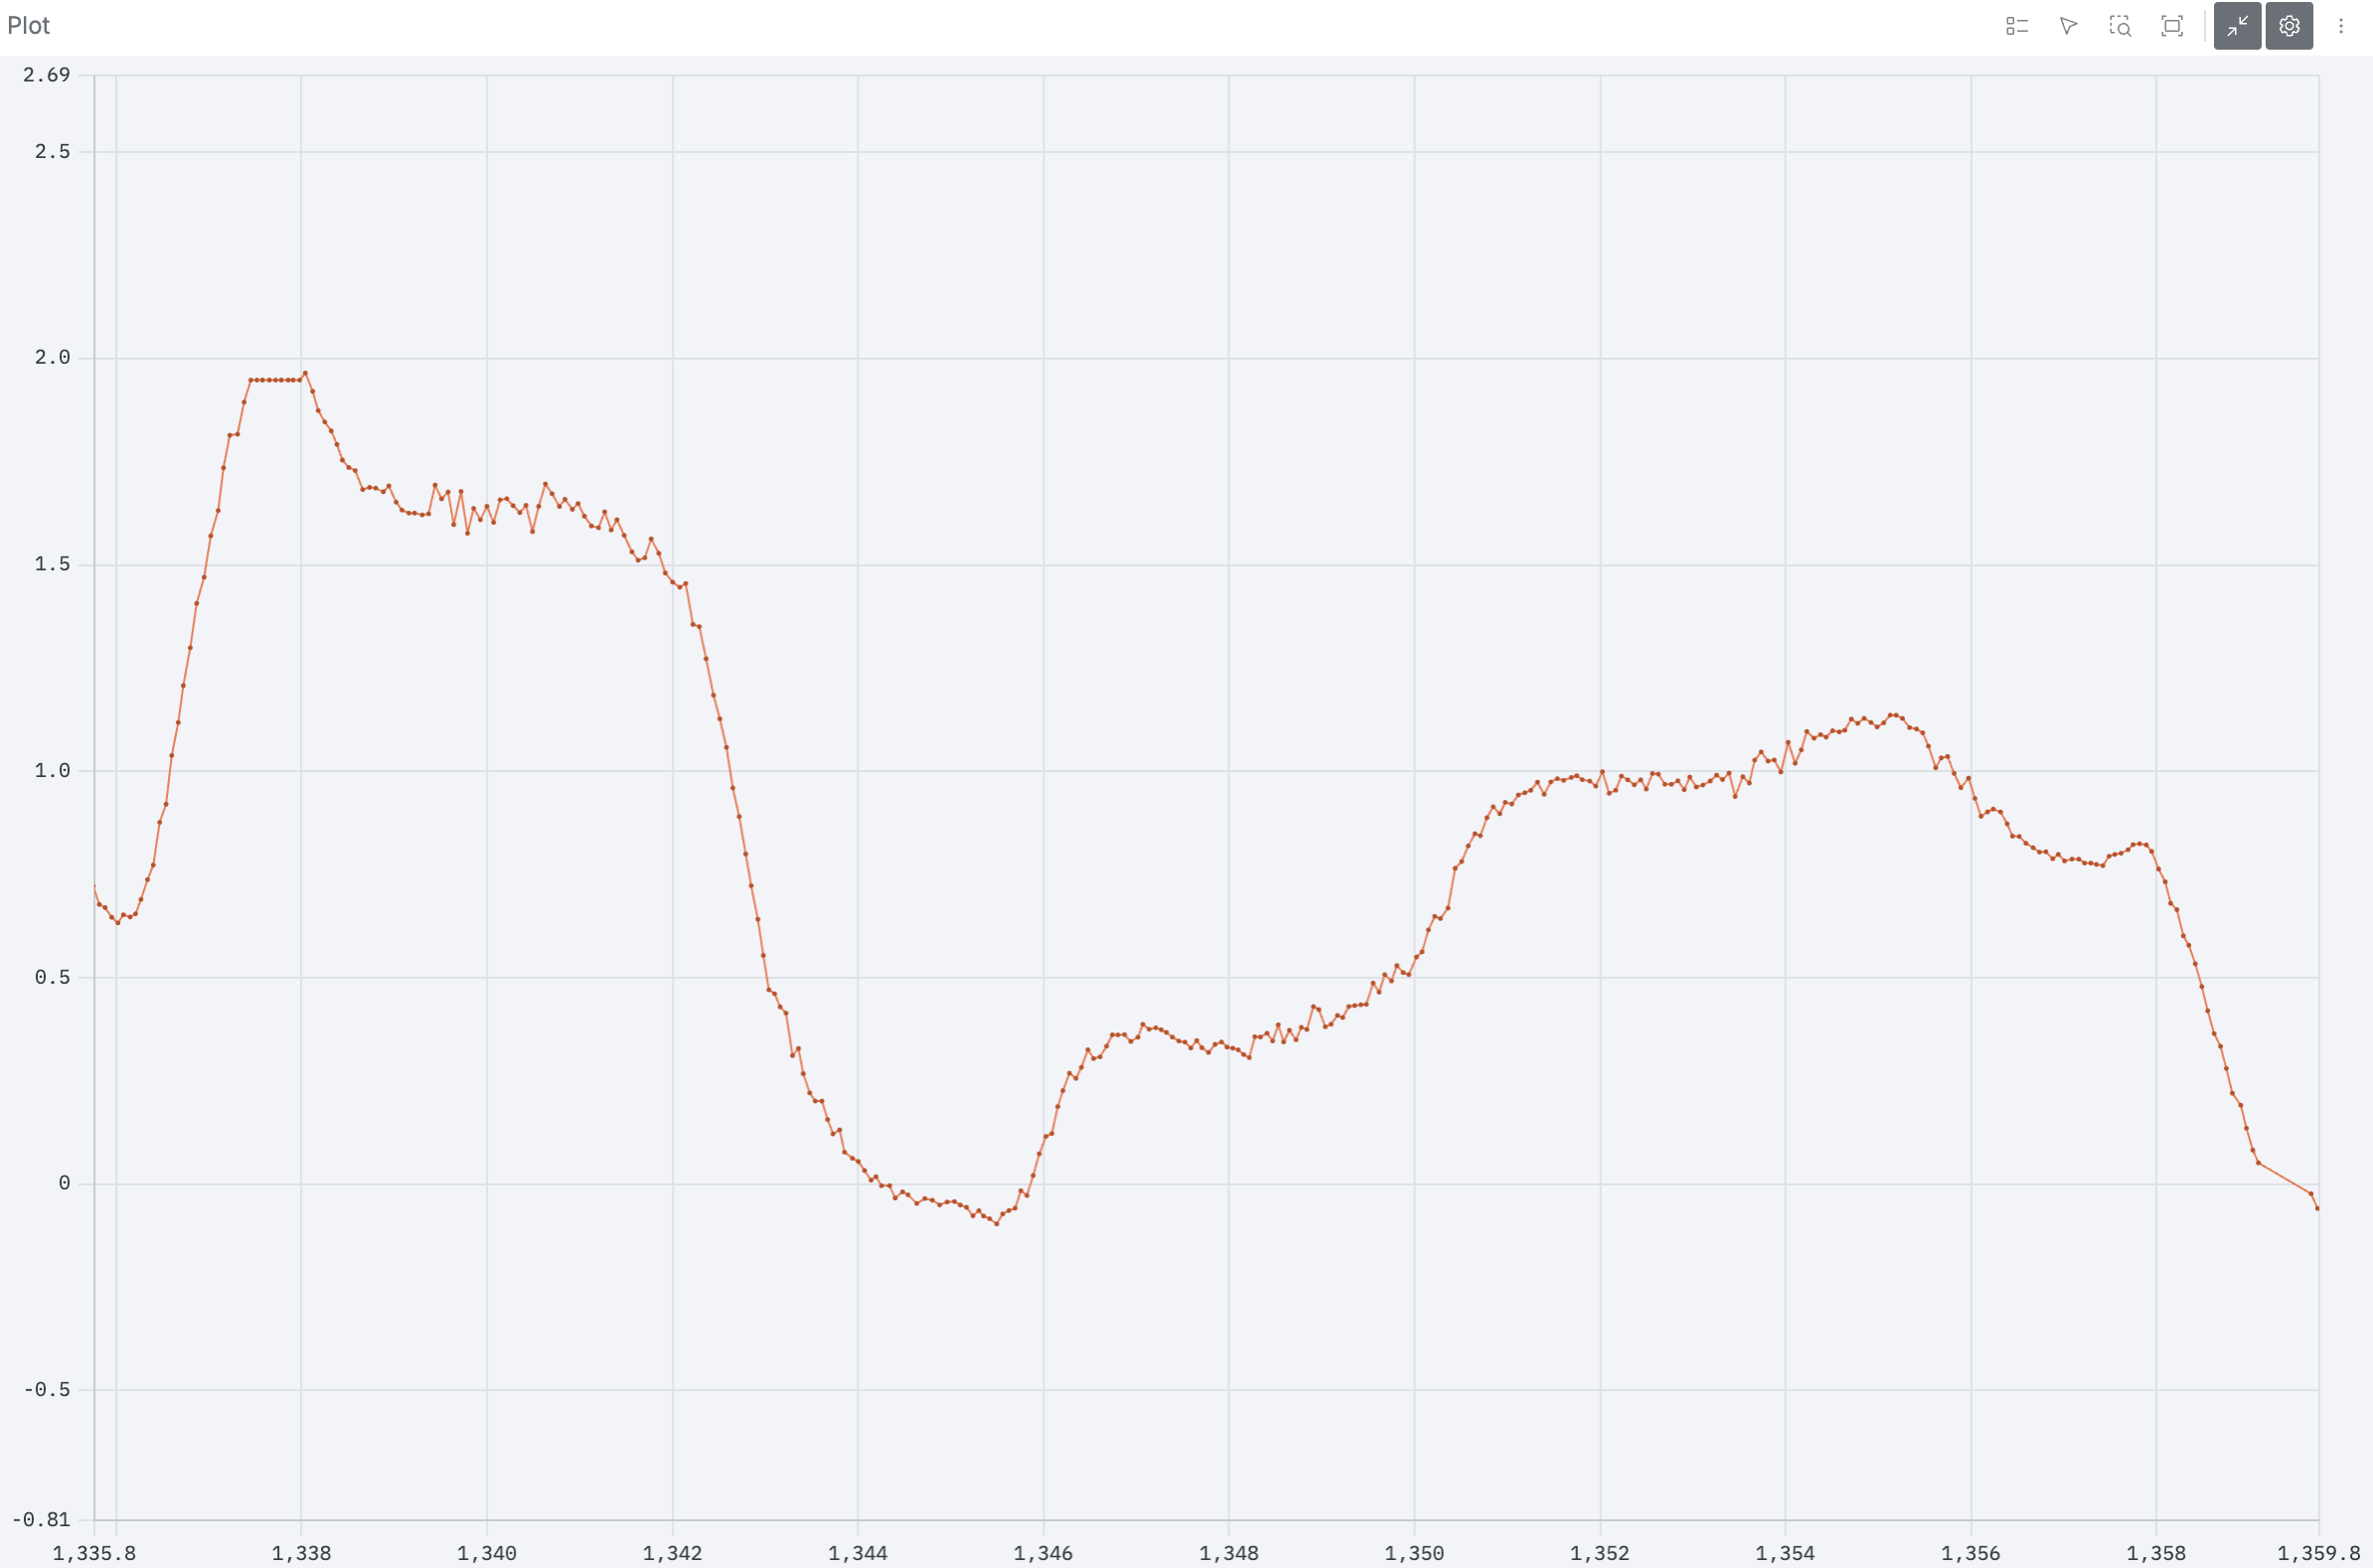
\includegraphics[width=\textwidth, trim={0 0 0 0}, clip]{immagini/log_non_distorto.png}
		\caption{Log con camera global shutter.}
		\label{fig:log_global_shutter}
	\end{subfigure}
	\caption{Due esempi di log del valore di localizzazione X calcolato utilizzando una camera rolling e global shutter. Si nota subito come nella immagine a il valore subisca dei salti improvvisi, mentre nell'immagine b non sono presenti}
	\label{fig:log_rolling_global}
\end{figure}
Utilizzare una camera global shutter risolve completamente il problema, ma al netto di un costo economico maggiore. La camera scelta è basata sul sensore OV7251\footnote{\url{https://www.ovt.com/products/ov7251/}}: ha una risoluzione di 640x480 pixel, bianco e nero e ha un sensore global shutter.

\subsubsection{Parametri della camera in picamera2}
Il modulo Python \texttt{picamera2} permette di configurare la camera a piacere. I parametri scelti per il sistema sono i seguenti:
\begin{itemize}
	\item la configurazione utilizata è la \texttt{create\_video\_configuration}, perché consente di avere un flusso più continuo e costante.
	\item \texttt{size}: permette di impostare la risoluzione dell'immagine, senza tagliarla. Dopo varie prove, è stata scelta una risoluzione di 640×480 per il suo compromesso tra precisione e velocità di elaborazione dell'immagine per la VO.
	\item \texttt{format}: imposta il formato dell'immagine. È stato scelto \texttt{YUV420}, un formato molto leggero e comodo per estrarre l'immagine in bianco e nero.
	\item \texttt{buffer\_count}: impostato ad 1 per avere sempre l'ultima immagine catturata. In questo modo, il tempo tra la richiesta dell'immagine e la risposta resta costante.
	\item \texttt{ExposureTime}: rappresenta il tempo di esposizione del sensore alla luce. Impostando un valore troppo alto, l'immagine risulta troppo chiara e mossa; troppo basso, diventa scura e con delle imperfezioni, dovute dalla compensazione con l'aumento della sensibilità del sensore. Sono stati fatti dei test nell'ambiente in cui il sistema lavora ed è stato scelto un valore di 1500\(\mu s\).
	\item \texttt{FrameDurationLimits}: imposta un limite minimo e massimo dell'intervallo temporale tra un frame e un'altro, quindi imposta il frame rate della camera. È stato impostato a 16666\(\mu s\) sia per il minimo che per il massimo.
\end{itemize}

\subsubsection{Calibrazione della camera}
La calibrazione della camera è un passaggio fondamentale per poter ottenere stime affidabili di posizione e posa del drone attraverso le immagini. Questo procedimento ci permette di ottenere due parametri principali:
\begin{itemize}
	\item Parametri intrinsechi: sono le caratteristiche interne e quelle geometriche del sensore e dell'ottica. Viene rappresentata attraverso una matrice 3x3 composta in questo modo: 
	\[
	\mathbf{K} = \begin{bmatrix} 
		f_x & 0 & c_x \\ 
		0 & f_y & c_y \\ 
		0 & 0 & 1 
	\end{bmatrix}
	\]
	Dove $f_x, f_y$ rappresentano la lunghezza focale della camera in pixel e $c_x, c_y$ sono le coordinate in pixel del centro ottico.
	\item Coefficienti di distorsione: sono dei parametri che rappresentano la distorsione radiale e tangenziale della camera, ovvero descrivono in che modo un obiettivo deforma i raggi luminosi, facendo apparire curve le linee rette. Il numero di questi parametri varia in base alla complessità dell'obiettivo e al modello matematico scelto.
\end{itemize}
Il metodo scelto per la calibrazione della camera è attraverso il modulo OpenCV. Per prima cosa, bisogna scattare delle foto da varie angolazioni di una scacchiera bianco nera, come quella in Fig. \ref{fig:calibration_chess}. Dopodiché, un programma analizzerà tutte le foto scattate e ne restituirà i parametri. È disponibile un esempio sul sito ufficiale di OpenCV \footnote{\url{https://docs.opencv.org/4.13.0/dc/dbb/tutorial_py_calibration.html}}.

\begin{figure}[!htbp]
	\centering
	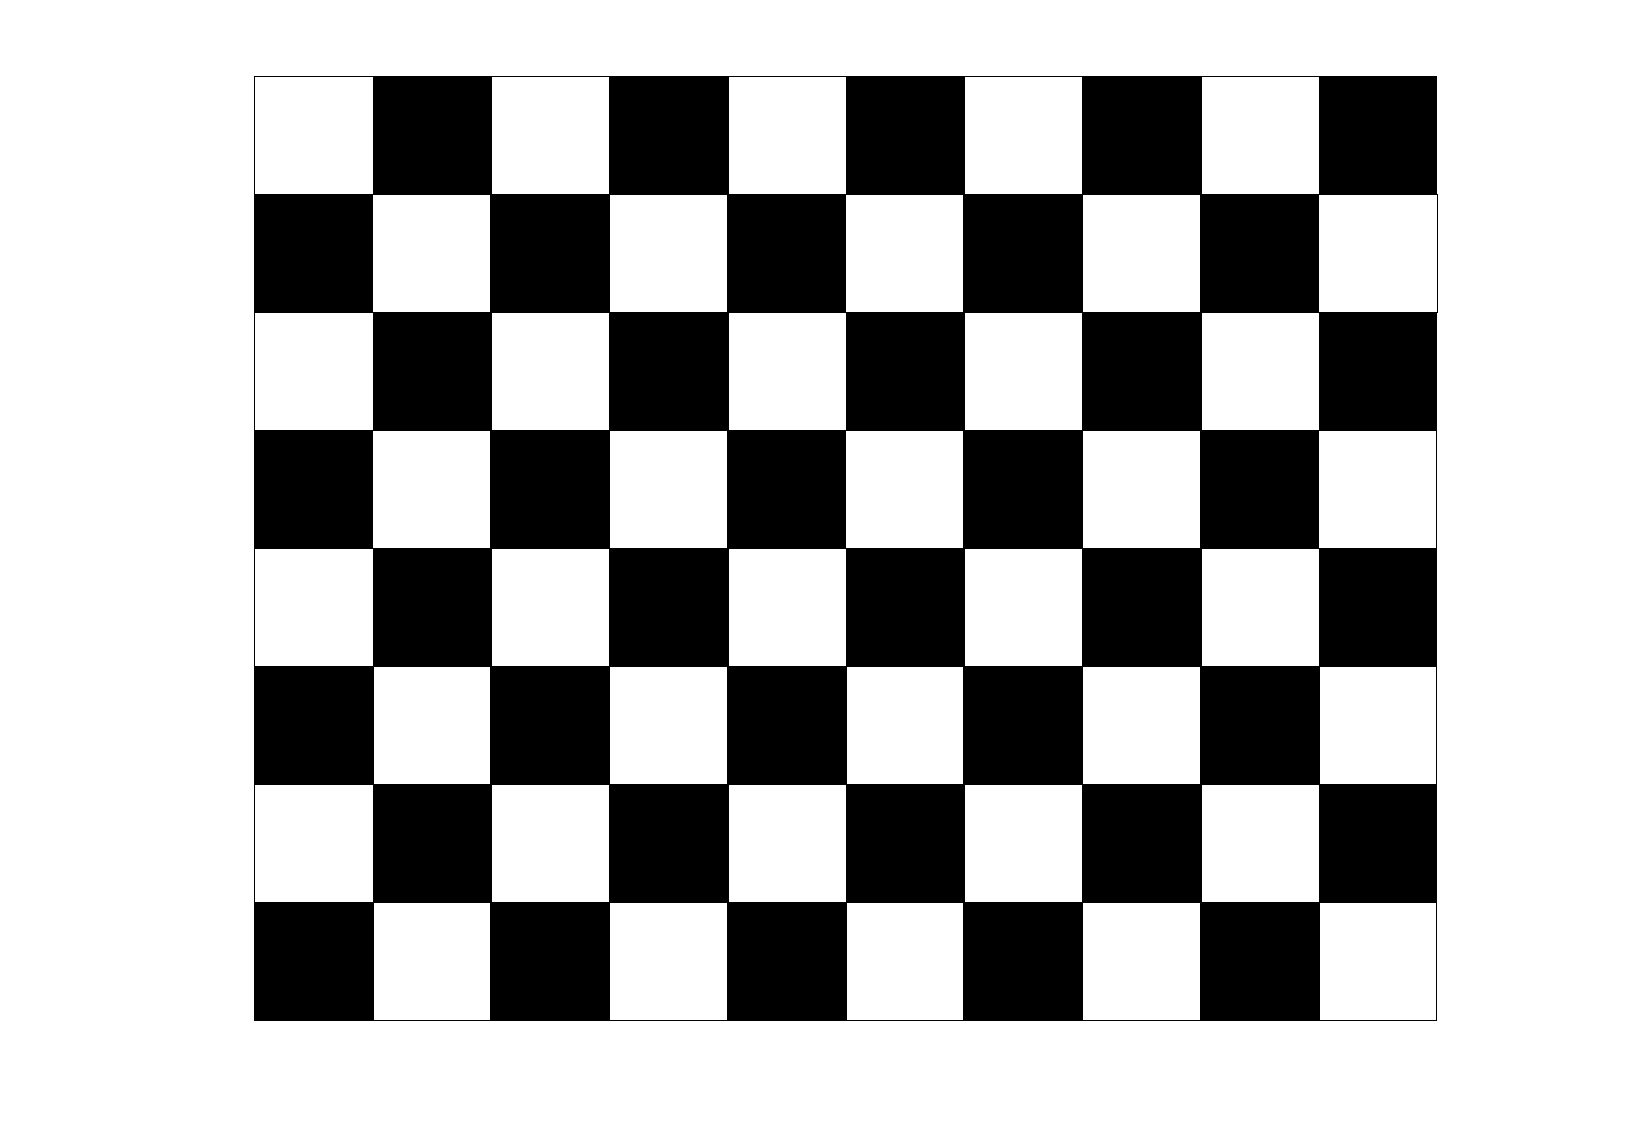
\includegraphics[width = 1\textwidth, trim={0 0 0 0}, clip]{immagini/chessboard-to-print.pdf}
	\caption{Scacchiera 7x9 usata per calibrare una camera. Il tipo di scacchiera viene calcolato contando gli angoli interni, non i quadrati.}
	\label{fig:calibration_chess}
\end{figure}